\documentclass[11pt,a4paper]{article}
\usepackage[margin=2.6cm]{geometry}
\usepackage{amsmath,amssymb,amsthm}
\usepackage{graphicx}
\usepackage{booktabs}
\usepackage{array}
\usepackage{xcolor}
\usepackage[colorlinks=true,linkcolor=blue!50!black,citecolor=blue!50!black,urlcolor=blue!50!black]{hyperref}
\usepackage{microtype}
\setlength{\emergencystretch}{3em}

\newtheorem{theorem}{Theorem}
\newtheorem{lemma}{Lemma}
\newtheorem{proposition}{Proposition}
\newtheorem{corollary}{Corollary}
\newtheorem{conjecture}{Conjecture}
\theoremstyle{remark}
\newtheorem{remark}{Remark}

\newcommand{\Exp}{\mathrm{Exp}}
\newcommand{\cv}{\mathrm{cv}}
\newcommand{\dd}{\,\mathrm{d}}
\newcommand{\eqd}{\stackrel{d}{=}}

\title{\bfseries An exact exponential fixed point and metastable shape manifolds in a
renormalization cascade of finite-time Lyapunov distributions:\\[2mm]
\large a two-class split of chaotic dynamics}
\author{Rajveer Kapoor\thanks{Corresponding author: \texttt{kapoorrajveer10@gmail.com}}\\[3pt]
{\normalsize Pathways School Noida}}
\date{July 2026}

\begin{document}
\maketitle

\begin{abstract}
\noindent
We study a renormalization cascade $T$ on distributions of finite-time Lyapunov exponents (FTLEs):
at each level, samples are replaced by mean-normalized absolute differences of independent pairs and a
maximum-likelihood tail exponent is read off. The operator arose in our own large-scale computational
study of double-pendulum chaos, where its limit $\alpha^*\!\approx\!4$ was conjectured to be a new
universal constant; here we give it an exact theory. The exponential distribution is the \emph{unique}
exact fixed point of $T$ (Puri--Rubin), with a closed-form reading
$\alpha^*_{\Exp}(f)=1+[\tfrac1f E_1(\ln\tfrac1f)]^{-1}=3.3494$ at $f=0.2$, confirmed to
$0.02\%$--$0.3\%$; and \emph{every} Gaussian bulk collapses in a single step to one universal
half-normal shape. Linearizing $T$ exactly, the symmetrization step halves excess kurtosis per level
--- which \emph{derives} the previously-empirical ``universal'' decay constant $r\approx1/2$ --- atop a
gapless, non-normal spectrum ($\mu(s)=2/(2-s)$ over a unit-diagonal polynomial tower) whose measured
consequence is algebraic relaxation and metastable plateaus. The celebrated ``$\alpha^*\!\approx\!4$''
is therefore a plateau reading of a marginal flow, not an asymptotic constant, and the operator is
provably not a tail-index estimator. What survives is sharper: a \emph{two-class split of chaotic
dynamics}. Across eleven FTLE ensembles from five systems, mixed-phase dynamics yields broad,
\emph{platykurtic} FTLE bulks that read strictly \emph{above} the exponential fixed point, while fully
chaotic, dissipative and near-regular dynamics yield \emph{leptokurtic} bulks that read \emph{below}
it --- a sign-perfect separation ($11/11$; sign test $p=0.001$; Cohen's $d=3.3$ on a
same-map/same-protocol control) with statistically zero within-class heterogeneity. An out-of-sample
H\'enon--Heiles sweep, predicted in advance, flips its matched-null excess exactly where phase space
turns from a thin chaotic web to a mixed sea. The FTLE distribution's shape, read against an exactly
known reference point, is a cheap and sensitive probe of a system's ergodic architecture.
\end{abstract}

\vspace{4pt}\noindent\textbf{Keywords:} finite-time Lyapunov exponents; chaotic Hamiltonian dynamics;
mixed phase space; renormalization fixed point; Chirikov standard map; double pendulum; extreme-value
theory; universality class; metastable plateaus

\tableofcontents

%======================================================================
\section{Introduction}\label{sec:intro}

The distribution of finite-time Lyapunov exponents (FTLEs) is one of the most information-rich
observables of a chaotic system. Its mean estimates the leading Lyapunov exponent
\cite{oseledec,benettin}; its width and shape encode the fluctuations of local expansion rates and,
through large-deviation theory, the multifractality of the invariant measure
\cite{grassberger,prasad,pikovsky,ott}. In Hamiltonian systems with mixed phase space, trajectories
intermittently trapped near regular islands depress their finite-time exponents, producing
long-lived non-Gaussian structure \cite{zaslavsky,meiss}; the associated algebraic decay of
Poincar\'e recurrences is itself conjectured universal \cite{chirikovshep,cristadoro}.

This paper concerns a specific, deceptively simple \emph{renormalization cascade} on FTLE
distributions that emerged from our own large-scale computational study of double-pendulum chaos
\cite{shinbrot,stachowiakNote} (hereafter, the \emph{source program}). Starting from the chaotic
subset of an FTLE sample, the operator
repeatedly (i) fits a maximum-likelihood power-law exponent to the upper tail, and (ii)
coarse-grains the sample by replacing it with mean-normalized absolute differences of independent
pairs. The per-level exponents $\alpha_k$ were observed to converge geometrically to a limit
$\alpha^*\!\approx\!4$, robust across hundreds of double-pendulum parameter combinations, and this
value --- together with a companion level-zero exponent $\alpha_0\!\approx\!8.3$ --- was conjectured
to be a new universal constant of chaotic Hamiltonian dynamics. We subsequently re-measured this
claim family ourselves at $n=5\times10^{5}$--$5\times10^{6}$ per system, which sharpened the empirical
picture in two directions: the
$\alpha^*$ landscape over double-pendulum parameter space is statistically \emph{flat} (no ridge
structure survives a noise null), and a class of dynamically distinct systems --- the dissipative
Lorenz-63 attractor, the fully chaotic standard map at $K=5$, and a near-regular coupled quartic
oscillator --- cluster at a sharply \emph{different} fixed point, $\alpha^*\!\approx\!3.0$--$3.3$,
while mixed-phase systems (the double pendulum family and the standard map just above the
connectedness threshold, $K=1$) cluster near $3.9$--$4.4$ \cite{note-registry}.

Two questions therefore demanded an answer. \emph{What does this operator actually measure?} And
\emph{is the two-class structure a property of the dynamics or of the statistics?} We answer both.

\paragraph{Contributions.}
\begin{enumerate}\itemsep2pt
\item \textbf{Exact fixed point (Theorem~\ref{thm:exp}).} The exponential distribution is an exact
fixed point of the cascade map, including its mean normalization; by the characterization theorem of
Puri and Rubin \cite{purirubin} it is the \emph{unique} distribution satisfying
$|X-Y|\eqd X$. The folding identity behind it is elementary and, to our knowledge, has not
previously been connected to Lyapunov statistics.
\item \textbf{Closed-form readings (Propositions~\ref{prop:reading}, \ref{prop:gauss0}).} The
maximum-likelihood tail exponent that the pipeline assigns to the exponential fixed point is
derived in closed form, $\alpha^*_{\Exp}(f)=1+[\tfrac1f E_1(\ln\tfrac1f)]^{-1}$
($=3.3494$ at $f=0.2$), and confirmed numerically to $0.02\%$. Companion formulas for the
half-normal ($4.4448$), the uniform ($9.6417$), and a first-order level-zero law for Gaussian bulks,
$\alpha_0 \approx 1 + (\cv^{-1}+z_f)/m_f$, are likewise derived and confirmed.
\item \textbf{Universal Gaussian collapse (Theorem~\ref{thm:gauss}).} Because the location parameter
cancels in pair differences, \emph{every} Gaussian bulk is mapped in one cascade step to the same
half-normal shape. All Gaussian-seeded flows therefore coincide from level one onward --- measured:
$\alpha_1 = 4.448$--$4.455$ across coefficients of variation $0.05$--$0.33$ --- and define a single
slow relaxation manifold toward the exponential fixed point.
\item \textbf{Metastability (\S\ref{sec:metastable}).} Deep cascades ($n=1.6\times10^{7}$, 20
levels) show the Gaussian-seeded flow's Kolmogorov distance to the exponential collapsing from
$0.34$ to $0.03$ within five levels and then \emph{stalling} at $0.02$--$0.03$ for at least eight
more, while the fitted exponent drifts slowly ($\approx-0.04$ per level) through precisely the range
in which the empirical ``constants'' were reported. The $n$-dependence of the double-pendulum
plateau ($4.64 \to 4.12 \to 3.88$ for $n=5\times10^4 \to 5\times10^5 \to 5\times10^6$) rides this
drift. ``$\alpha^*\approx4$'' is a metastable plateau reading, not an asymptotic constant.
\item \textbf{The operator is not a tail estimator (\S\ref{sec:calibration}).} Genuine Pareto tails
are asymptotically conserved by the cascade (Proposition~\ref{prop:conserve}) but are \emph{not}
recovered by the finite-window fit: pure Pareto inputs with survival indices $2.5/4/6$ read
$2.4/2.7/2.9$ after one step. Any interpretation of $\alpha^*$ as a physical tail index is
untenable.
\item \textbf{The two-class split is real, and its mechanism is identified
(\S\ref{sec:twoclass}).} Across eleven ensembles from five systems, mixed-phase dynamics produces
broad, near-symmetric, \emph{platykurtic} FTLE bulks (excess kurtosis $-1.0$ to $-1.3$) that read
strictly above the exponential fixed point, while non-mixed dynamics produces narrow or skewed
\emph{leptokurtic} bulks (excess kurtosis $+1.3$ to $+43$) that read below it. A per-system
matched-Gaussian null --- a folded Gaussian with the system's own mean and variance --- gives a
sign-perfect separation ($11/11$ ensembles, $p=0.001$; $8/8$ systems, $p=0.008$). The contrast
survives the sharpest available control: the same map, integrator, horizon and $n$ at $K=1$
(mixed) versus $K=5$ (fully chaotic). A random-effects meta-analysis finds within-class
heterogeneity indistinguishable from zero ($\tau^2$ CI $[0, 0.012]$, Cochran $p=0.36$), so the split
is a \emph{discrete class boundary}, not a soft gradient.
\item \textbf{Exact linearization; the decay constant $r \approx 1/2$ derived
(\S\ref{sec:linear}).} The symmetrization step $A - B$ annihilates all odd cumulants and rescales
the standardized cumulant of order $2m$ by exactly $2^{1-m}$: excess kurtosis halves per step,
verified on pendulum data to three decimals. This derives the source program's second empirical
constant --- the ``nearly universal'' geometric decay $r \approx 0.46$--$0.51$ of the cascade fit,
i.e.\ $\log_2 r \approx -1$. The linearized operator at the fixed point has the closed-form
eigenfamily $\mu(s) = 2/(2-s)$ and a unit-diagonal triangular action on polynomials: no spectral
gap, hence \emph{algebraic} relaxation (measured $d_k \sim k^{-0.5}$) and metastable plateaus.
\item \textbf{What the pendulum constants are: frozen ensemble statistics
(\S\ref{sec:ensemble}).} Across horizons $T = 5$--$200$ the chaotic-subset FTLE variance does not
decay at all ($\beta = -0.014$, fit RMS $0.002$, against $\mathrm{var} \sim T^{-\beta}$; CLT
self-averaging predicts $\beta = 1$). The canonical release ensemble (uniform angles, zero
velocity) is revealed as a mixture over energy shells --- $E(\theta)$ explains
$\eta^2 = 0.41$--$0.43$ of the variance --- and over invariant components within shells (the
remaining $59\%$, equally frozen). Energy bands internally recapitulate the entire two-class
taxonomy within one system.
\item \textbf{Out-of-sample validation: H\'enon--Heiles across its transition
(\S\ref{sec:hh}).} A fresh symplectic-variational implementation of the H\'enon--Heiles system
(named in advance as a falsifiable prediction of the classifier, before the experiment was built)
shows the matched-null excess flipping sign precisely where phase space transitions from a thin
chaotic web to a fat mixed sea, with the platykurtic signature switching on alongside it.
\end{enumerate}

Section~\ref{sec:operator} develops the exact theory; \S\ref{sec:protocols} describes systems,
integrators, and statistical protocols; \S\ref{sec:calibration} calibrates the operator on synthetic
ensembles; \S\ref{sec:twoclass} presents the two-class result; \S\ref{sec:metastable} quantifies
metastability and demystifies the original constants; \S\ref{sec:mechanism} discusses the dynamical
mechanism and predictions; \S\ref{sec:numbers} is a number-theoretic audit of every constant
appearing in this work; \S\ref{sec:conclusions} concludes. Appendices contain derivations, data
provenance, the full calibration table, and estimator pathologies.

%======================================================================
\section{The cascade operator and its exact structure}\label{sec:operator}

\subsection{Definitions}

Let $x = (x_1,\dots,x_n)$, $x_i>0$, be an FTLE sample (the ``chaotic subset'', $x_i > 0.01$
throughout). The cascade is built from two ingredients.

\paragraph{The reading $\eta_f$.} For tail fraction $f\in(0,1)$ define the Clauset--Hill
maximum-likelihood tail exponent \cite{hill,clauset}
\begin{equation}\label{eq:estimator}
\eta_f(x) \;=\; 1 + \frac{n_u}{\sum_{x_i \ge u}\ln (x_i/u)},
\qquad u = x_{(\lceil (1-f) n\rceil)},
\end{equation}
with $x_{(\cdot)}$ the order statistics and $n_u = \#\{x_i \ge u\}$; $u$ is the empirical
$(1-f)$-quantile. For a distribution $F$ we write $\eta_f(F)$ for the $n\to\infty$ limit,
\begin{equation}\label{eq:etaF}
\eta_f(F) = 1 + \Bigl[\,\mathbb{E}\bigl(\ln (X/u_F)\,\big|\,X \ge u_F\bigr)\Bigr]^{-1},
\qquad u_F = F^{-1}(1-f).
\end{equation}

\paragraph{The coarse-graining $T$.} Given the level-$k$ sample $x^{(k)}$ of size $n_k$, form
$n_{k+1} = \lfloor n_k/2\rfloor$ independent pairs $(a_i,b_i)$ and set
\begin{equation}\label{eq:T}
x^{(k+1)}_i \;=\; \frac{\lvert a_i - b_i\rvert}{\overline{x^{(k)}}},
\end{equation}
discarding zeros; $\overline{x^{(k)}}$ is the level mean. On distributions, $T$ maps the law of $X$
to the law of $|A-B|/\mathbb{E}X$ with $A,B \sim X$ independent. The \emph{cascade} records
$\alpha_k = \eta_f(x^{(k)})$, $k=0,1,2,\dots$ (default $f=0.2$), halving the sample each level, and
the original pipeline summarizes the sequence by a three-parameter geometric fit
$\alpha_k \simeq \alpha^* + C r^k$ (Appendix~\ref{app:pathologies} documents when this fit is and is
not well-posed; we use a fit-free \emph{plateau} statistic, the median of $\alpha_k$ over the last
well-sampled levels, alongside it).

\subsection{Scale invariance}

\begin{lemma}[scale invariance]\label{lem:scale}
For every $c>0$ and every sample, $\eta_f(cx) = \eta_f(x)$; consequently $T$ acts on distribution
\emph{shapes} and the cascade $\{\alpha_k\}$ is invariant under any positive rescaling of the input.
\end{lemma}

\begin{proof}
The threshold $u$ in \eqref{eq:estimator} is an empirical quantile, hence equivariant ($u \mapsto
cu$), and the estimator depends on the data only through the ratios $x_i/u$. The mean-normalization
in \eqref{eq:T} then fixes the scale of every level, so only the shape of the input law matters.
(This reproduces, as a special case, the bit-exact agreement of the published pipeline under
mean-, median- and standard-deviation-normalization of its input.)
\end{proof}

\subsection{The exponential fixed point and its uniqueness}

\begin{theorem}[exact fixed point]\label{thm:exp}
Let $A,B \sim \Exp(\theta)$ be independent. Then $\lvert A-B\rvert \sim \Exp(\theta)$, and
$\Exp(1)$ is an exact fixed point of $T$, including its mean normalization. Moreover, among
distributions on $[0,\infty)$ (excluding the degenerate case), $\Exp$ is the \emph{unique} law
satisfying $\lvert A - B\rvert \eqd A$ \emph{(Puri--Rubin \cite{purirubin})}.
\end{theorem}

\begin{proof}
For the folding identity: $A-B$ has the Laplace density $\tfrac{\theta}{2}e^{-\theta|z|}$, so
$|A-B|$ has density $\theta e^{-\theta z}$ on $z>0$, i.e.\ is $\Exp(\theta)$ again. For
$\theta = 1$, $\mathbb{E}A = 1$, so the normalization in \eqref{eq:T} is by unity and
$T(\Exp(1)) = \Exp(1)$ exactly. Uniqueness of the unit-scale fixed-point equation is Theorem~1 of
\cite{purirubin}. (An equivalent route: $|A-B|$ conditioned on $A\ne B$ is, by memorylessness, the
excess of $A$ over an independent copy, and the exponential is the unique memoryless law.)
\end{proof}

\begin{remark}
Fixed shapes of $T$ satisfy the more general equation $|A-B| \eqd cX$ with
$c = \mathbb{E}|A-B|/\mathbb{E}X \in (0,1]$, and $c=1$ forces the exponential by
\cite{purirubin}. We are not aware of a classification for $c<1$; among the seventeen synthetic
families tested below we find no other attracting fixed shape, only \emph{slow manifolds}
(\S\ref{sec:metastable}). A rigorous basin/spectral analysis of $T$ at $\Exp$ is an open problem we
commend to the reader (\S\ref{sec:mechanism}).
\end{remark}

\subsection{Closed-form readings}

\begin{proposition}[the exponential reading]\label{prop:reading}
For $X \sim \Exp(1)$ and tail fraction $f$,
\begin{equation}\label{eq:reading}
\eta_f(\Exp) \;=\; 1 + \Bigl[\tfrac1f\,E_1\bigl(\ln \tfrac1f\bigr)\Bigr]^{-1},
\qquad E_1(u) = \int_u^\infty \frac{e^{-s}}{s}\dd s .
\end{equation}
In particular $\eta_{0.1} = 4.0874$, $\eta_{0.2} = 3.3494$, $\eta_{0.3} = 2.9058$.
\end{proposition}

\begin{proof}
$u_F = \ln(1/f)$. By memorylessness, $X-u_F \,|\, X>u_F \sim \Exp(1)$, so with $E \sim \Exp(1)$,
$\mathbb{E}\ln(X/u_F \,|\, X>u_F) = \mathbb{E}\ln(1+E/u_F) = \int_0^\infty e^{-t}\ln(1+t/u_F)\dd t
= e^{u_F}E_1(u_F)$ after one integration by parts; and $e^{u_F} = 1/f$. Insert into
\eqref{eq:etaF}.
\end{proof}

Because $\Exp$ is a fixed point, \eqref{eq:reading} is simultaneously the level-zero reading and
the $k\to\infty$ reading of an exponential seed --- a sharp, parameter-free prediction. It is
confirmed to $0.02\%$--$0.3\%$ (Table~\ref{tab:analytic}); the flatness of the measured exponential
cascade over 14 levels (5M seed: $3.3462, 3.3455, 3.3445, 3.3495, \dots$) is the fixed-point
signature in its rawest form.

\begin{table}[t]
\centering\small
\caption{Derived readings versus measurement. ``Level-0'' entries are single-level readings of
$5\times10^{5}$-point samples; the 5M entry is the geometric-fit limit of a full 14-level cascade on
$5\times10^{6}$ exponential points. Gaussian level-1 entries verify Theorem~\ref{thm:gauss}
(three independent seeds and four widths).}
\label{tab:analytic}
\begin{tabular}{llll}
\toprule
quantity & derived & measured & rel.\ dev.\\
\midrule
$\eta_{0.1}(\Exp)$ & $4.0874$ & $4.0883$ & $0.02\%$\\
$\eta_{0.2}(\Exp)$ & $3.3494$ & $3.3605$; $3.3507$ (5M) & $0.33\%$; $0.04\%$\\
$\eta_{0.3}(\Exp)$ & $2.9058$ & $2.9110$ & $0.18\%$\\
$\eta_{0.2}(\text{half-normal})$ & $4.4448$ & $4.4494,\ 4.4473,\ 4.4572$ & $\le 0.3\%$\\
$\eta_{0.2}(\text{uniform})$ & $9.6417$ & $9.6135$ & $0.29\%$\\
Gaussian level-1 ($\cv = 0.05/0.1/0.33$) & $4.4448$ & $4.448/4.450/4.455$ & $\le 0.23\%$\\
\bottomrule
\end{tabular}
\end{table}

\subsection{Universal Gaussian collapse}

\begin{theorem}[one-step collapse of Gaussian bulks]\label{thm:gauss}
Let $X = \lvert N(\mu,\sigma^2)\rvert$ with $\mu/\sigma \to \infty$ (negligible folded mass). Then
$T(X)$ is the half-normal law $\lvert N(0, 2\sigma^2)\rvert$ rescaled by $1/\mu$ --- \emph{independent
of $\mu/\sigma$ up to scale}. Hence by Lemma~\ref{lem:scale} all Gaussian bulks share a single
cascade flow from level 1 onward, beginning at $\alpha_1 = \eta_f(\text{half-normal})$
($=4.4448$ at $f = 0.2$).
\end{theorem}

\begin{proof}
$A - B \sim N(0, 2\sigma^2)$ exactly --- the means cancel. Folding and normalizing by
$\mathbb{E}X \approx \mu$ gives the claim; the correction is $O(\Phi(-\mu/\sigma))$.
\end{proof}

This explains, at a stroke, why the empirical study found the \emph{same} convergence pattern across
so many parameter combinations: any near-Gaussian FTLE bulk forgets its width in one cascade step.
Measured level-1 values across seeds and widths agree with the derived $4.4448$ to
$\le0.3\%$ (Table~\ref{tab:analytic}); at $\cv = 0.6$ the folded mass ($\approx 5\%$) shifts
$\alpha_1$ to $4.60$, quantifying the stated correction.

\begin{proposition}[first-order level-zero law for Gaussian bulks]\label{prop:gauss0}
For $X = |N(\mu,\sigma^2)|$ with $\cv = \sigma/\mu$ small, writing $z_f = \Phi^{-1}(1-f)$ and
$m_f = \varphi(z_f)/f - z_f$,
\begin{equation}\label{eq:gauss0}
\eta_f(X) \;\approx\; 1 + \frac{\cv^{-1} + z_f}{m_f},
\qquad (z_{0.2}, m_{0.2}) = (0.8416,\ 0.5582).
\end{equation}
\end{proposition}

\begin{proof}
To first order in $\sigma/u$, $\ln(x/u) \approx (x-u)/u$; the Gaussian mean excess above the
$(1-f)$-quantile is $\sigma m_f$ and $u = \mu + \sigma z_f$.
\end{proof}

On \emph{exact} folded-Gaussian ensembles matched to each dynamical system (\S\ref{sec:twoclass})
this law predicts $\alpha_0$ to $3$--$5\%$ across two orders of magnitude of $\cv$ (predicted/measured:
$75.5/76.4$ at $\cv=0.025$; $32.3/33.2$ at $0.060$; $13.0/13.7$ at $0.171$; $5.5/5.8$ at $0.59$).
Its physical import: \emph{the level-zero exponent $\alpha_0$ is a bulk-width statistic}, not a tail
exponent --- $\alpha_0 \approx 8$ corresponds to nothing deeper than $\cv \approx 0.6$--$0.7$ bulk
via \eqref{eq:gauss0} corrected for the platykurtic shape (\S\ref{sec:twoclass}).

\subsection{Tail conservation --- and why it is not realized}

\begin{proposition}[asymptotic conservation of regularly varying tails]\label{prop:conserve}
If $P(X > x) = L(x)\,x^{-a}$ with $a > 1$ and $L$ slowly varying, then $T(X)$ has a regularly
varying tail with the \emph{same} index $a$.
\end{proposition}

\begin{proof}
For independent $A, B \sim X$ and $x \to \infty$,
$P(A - B > x) = \mathbb{E}_B\,P(A > x + B) \sim P(A > x)$ by dominated convergence
($B \ge 0$, $\mathbb{E}B < \infty$), and symmetrically for $B - A$; so
$P(|A-B| > x) \sim 2 P(A > x)$, which is regularly varying of index $-a$. Normalization is a
rescaling (Lemma~\ref{lem:scale}).
\end{proof}

One might conclude the cascade limit \emph{measures} $a$. It does not. The finite window
($f = 0.2$) reads the post-differencing \emph{bulk}: pure Pareto seeds with survival indices
$a = 2.5 / 4 / 6$ (level-0 readings $3.5 / 5.0 / 7.0$, i.e.\ $a{+}1$ as expected) collapse after a
single differencing step to flat sequences reading $2.4 / 2.7 / 2.9$ --- far below $a + 1$ and only
weakly ordered in $a$ (\S\ref{sec:calibration}, Fig.~\ref{fig:conservation}). Bulk-plus-tail
mixtures behave likewise. \emph{The operator is a bulk-shape reader; it is not a tail-index
estimator at any practical window.} Claims that cascade limits equal raw tail exponents are thereby
foreclosed --- consistently, direct Hill estimates of the same ensembles' raw upper tails give
values ($\sim$11--22) unrelated to any cascade reading.

\subsection{The linearized cascade: exact cumulant flow and a gapless, non-normal
spectrum}\label{sec:linear}

Two exact structures govern the approach to the fixed point.

\begin{proposition}[cumulant flow of the symmetrization step]\label{prop:cumulant}
Let $A, B$ be iid with cumulants $\kappa_n$ and let $D = A - B$. Then every odd cumulant of $D$
vanishes, and the standardized even cumulants transform as
\begin{equation}
\frac{\kappa_{2m}(D)}{\kappa_2(D)^{m}} \;=\; 2^{\,1-m}\,
\frac{\kappa_{2m}(A)}{\kappa_2(A)^{m}},
\qquad m = 1, 2, \dots
\end{equation}
In particular the excess kurtosis \emph{halves} exactly ($m=2$), the standardized sixth cumulant is
quartered, and skewness is annihilated.
\end{proposition}

\begin{proof}
Cumulants of independent sums add and are homogeneous: $\kappa_n(A - B) = \kappa_n(A) +
(-1)^n \kappa_n(B) = (1 + (-1)^n)\,\kappa_n$. Divide by $\kappa_2(D)^m = (2\kappa_2)^m$.
\end{proof}

Measured on the double-pendulum ensemble ($n = 5\times10^{5}$, level 0):
excess kurtosis of the signed differences $= -0.6442$ against the predicted
$-1.2896/2 = -0.6448$, with skewness $10^{-4}$; the identity holds at every level and for every
seed tested within sampling error (Appendix~\ref{app:data} scripts). Its dynamical consequence:
in the early cascade, where the deviation from the fixed point is carried by low-order cumulants,
the fitted geometric ratio of the exponent sequence is pinned near $1/2$. This \emph{derives} the
source program's second celebrated constant --- a decay rate reported as ``$r \approx 0.46$,
nearly constant across all systems'' (canonical fit $0.5061$; legacy published $0.4565$; 49-config
mean $0.4595$; our synthetic families $0.48$--$0.67$ on early windows), i.e.\
$\log_2 r \approx -1$ with computable corrections from higher cumulants and the folding step.

\begin{proposition}[linearization at the fixed point]\label{prop:linop}
Write level densities as $e^{-z}\bigl(1 + \varepsilon h(z)\bigr)$. To first order in
$\varepsilon$, one cascade step acts (modulo the rank-one normalization terms) by
\begin{equation}\label{eq:linop}
(L_0 h)(z) \;=\; 2\int_0^\infty e^{-2x}\, h(x + z)\,\dd x ,
\end{equation}
with the closed-form eigenfamily
\begin{equation}
h_s(z) = e^{s z}, \qquad \mu(s) = \frac{2}{2 - s}, \quad s < 1,
\end{equation}
and a triangular action with \emph{unit diagonal} on the polynomial tower:
$L_0[z^m] = z^m + (\text{lower order})$ for every $m$.
\end{proposition}

\begin{proof}
With $p(x) = e^{-x}(1 + \varepsilon h(x))$, the density of $|A - B|$ at $z > 0$ is
$2\int_0^\infty p(x) p(x + z)\dd x = e^{-z}\bigl[1 + \varepsilon\bigl(2c_h + (L_0h)(z)\bigr)\bigr] +
O(\varepsilon^2)$ with $c_h$ a constant absorbed by normalization. For $h_s$:
$2\int_0^\infty e^{-2x} e^{s(x+z)}\dd x = \tfrac{2}{2-s} e^{sz}$. For $z^m$, expand
$(x + z)^m$ and integrate term by term; the $z^m$ coefficient is $2\int_0^\infty e^{-2x}\dd x = 1$.
\end{proof}

Numerically (discretized kernel, $900$ points): $\mu(s)$ at $s = -0.5, -1, -2, -4$ measures
$0.8008$, $0.6677$, $0.5013$, $0.3353$ against the exact $0.8$, $\tfrac23$, $0.5$, $\tfrac13$,
and the polynomial leading coefficient is $1.0007$. Three structural consequences follow. \emph{First},
the kernel in \eqref{eq:linop} is one-sided (Volterra-type): the operator is far from
self-adjoint, and finite discretizations are defective --- their matrix eigenvalues collapse toward
the diagonal and do not see the eigenfamily; the operator's behaviour is governed by its
pseudo-spectrum, not its spectrum. \emph{Second}, the unit diagonal on the polynomial tower means
there is \emph{no spectral gap below $1$}: linear stability is marginal. \emph{Third}, marginal
non-normal flows relax \emph{algebraically}, not geometrically --- exactly what is measured: the
Gaussian-seeded deep cascade's Kolmogorov distance to the fixed point follows
$d_k \sim k^{-\theta}$ with $\theta = 0.55$--$0.58$ (log--log RMS $3\times$ smaller than the best
geometric fit); an independent uniform-seeded run ($n = 8\times10^{6}$) is compatible, and even
read geometrically decays no faster than $0.88$ per level. The metastable plateaus of
\S\ref{sec:metastable} are the quantitative face of this gapless linearization: fast transient
(cumulant halving, $r \approx 1/2$) followed by marginal drift ($k^{-1/2}$-type), so that
\emph{every} finite-depth experiment reads a plateau.

%======================================================================
\section{Systems, data and statistical protocol}\label{sec:protocols}

\paragraph{Dynamical systems.} We analyze eleven FTLE ensembles from five systems.
(i)~\emph{Double pendulum} (planar, equal-mass baseline; dimensional Lagrangian convention,
$g = 9.81$): FTLEs by the Benettin two-trajectory method \cite{benettin} with horizon $T = 15$\,s,
renormalization interval $\tau = 0.1$\,s, RK4 $\mathrm{d}t = 5\times10^{-3}$, perturbation
$10^{-7}$ on $\theta_1$, uniform-angle zero-velocity initial conditions; ensembles at
$n = 5\times10^{4}$, $5\times10^{5}$, $5\times10^{6}$, plus three geometric variants
($m$-ratio/$\ell$-ratio $= (0.5,1), (2,0.5), (0.5,2)$) at $5\times10^{5}$.
(ii)~\emph{Chirikov standard map} \cite{chirikov} at $K = 1$ (just above the connectedness
threshold $K_c = 0.9716$ \cite{greene}; mixed phase space) and $K = 5$ (islands destroyed; fully
chaotic), tangent-map Benettin with $10^{3}$ iterations, $n \approx 5\times10^{5}$.
(iii)~\emph{Lorenz-63} \cite{lorenz} at canonical parameters, joint state+tangent integration,
RK4 $\mathrm{d}t = 5\times10^{-3}$, $T = 100$, $\tau = 1$; mean FTLE $0.9042$ vs.\ the reference
$0.9056$ ($0.15\%$).
(iv)~\emph{Coupled quartic Hamiltonian} $H = \tfrac12(p_1^2{+}p_2^2) + \tfrac14(q_1^4{+}q_2^4) +
\tfrac\lambda2 q_1^2q_2^2$ at $E = 1$, $\lambda = 0.1, 0.2$ (near-regular at these couplings):
variational Benettin, 4th-order Yoshida symplectic integrator \cite{yoshida}
($\mathrm{d}t = 10^{-2}$, $T = 200$, $\tau = 10$), energy drift $|\Delta H/H| \le 5\times10^{-10}$.
Integrator cross-checks: measured RK4 energy-drift order $\mathrm{d}t^{4.79}$, Yoshida-4
$\mathrm{d}t^{4.00}$; FTLE differences between integrators are $\le 4\times10^{-4}$, immaterial
at our precision.

\paragraph{Chaotic subset and estimator.} Throughout, the chaotic subset is $x_i > 0.01$; the
estimator, tree and geometric fit are exactly \eqref{eq:estimator}--\eqref{eq:T} with $f = 0.2$
unless stated. Confidence intervals for cascade limits are bootstrap-through-the-tree (the base
sample is resampled and the \emph{entire} cascade re-run, $B = 250$--$1000$). Alongside the
geometric-fit $\alpha^*$ we report the fit-free \emph{plateau} statistic (median of $\alpha_k$ over
the last $\le 5$ levels with $n_k \ge 500$, $k \ge 2$); Appendix~\ref{app:pathologies} documents the
fit's failure modes (runaway to parameter bounds on flat or slowly-varying sequences) which the
plateau is immune to.

\paragraph{Provenance.} Every production array carries a manifest with SHA-256 checksum, seed,
integrator settings and moments; synthetic ensembles use fixed seeds. Scripts reproducing every
number and figure in this paper accompany it as supplementary material (Appendix~\ref{app:data}).

\paragraph{AI-use disclosure.} In line with COPE guidance and the preprint server's policy, the author
discloses that Anthropic's Claude large language models (Opus~4.6, 4.7 and 4.8, and principally
Fable~5) were used, through an agent-orchestration workflow, in the formulation of the research
programme, in performing and cross-checking computations, and in the analysis, drafting and editing of
this manuscript. All mathematical derivations, the numerical engines, and the reported results are the
author's own and were independently verified; consistent with COPE's position, the AI tools are not
authors and bear no responsibility for the content.

%======================================================================
\section{Calibration on synthetic ensembles}\label{sec:calibration}

Seventeen synthetic families ($n = 5\times10^{5}$ each; Appendix~\ref{app:battery} for the full
table) calibrate what the cascade responds to.

\paragraph{The exponential is flat; the fit can lie.} The $\Exp(1)$ cascade is flat at
$3.35$ for as many levels as sampling permits --- 14 levels at $n=5\times10^{6}$ with the geometric
fit returning $\alpha^* = 3.3507$, against the derived $3.3494$. At $n=5\times10^{5}$ the same flat
sequence defeats the three-parameter fit (it runs to its parameter bounds, reporting
$\alpha^* = 10.5$--$12$ with $r \to 1$); the plateau statistic returns $3.32$--$3.35$. All
quantitative claims below therefore quote the plateau alongside the fit
(Appendix~\ref{app:pathologies}).

\paragraph{One Gaussian flow.} Gaussian bulks of any width collapse onto the single half-normal-seeded
flow (Theorem~\ref{thm:gauss}): measured $\alpha_1 = 4.448$--$4.455$ across $\cv = 0.05$--$0.33$,
then $4.11 \to 3.94 \to 3.84 \to 3.81 \to \dots$ --- a slow descent toward the exponential reading,
still at $\approx 3.57$ ten levels in ($1.6\times10^{7}$-point seed) and $\approx 3.30$ at level 15
(Fig.~\ref{fig:flows}; \S\ref{sec:metastable}).

\paragraph{Skew selects the side of approach.} Right-skewed, leptokurtic families approach the
fixed point \emph{from below} and linger there: lognormal($\sigma{=}0.5$) descends to $3.10$--$3.24$;
lognormal($\sigma{=}1$) sits flat at $2.7$ for ten levels; Weibull($k{=}0.7$) ascends
$2.64 \to 3.3$. Bounded flat-topped inputs read \emph{high} (uniform: level-0 $9.61$, plateau
$\approx 4.1$). The taxonomy --- flat-topped/platykurtic above, peaked/skewed below, exponential
exactly at $\eta_f(\Exp)$ --- is the calibration key for \S\ref{sec:twoclass}.

\begin{figure}[t]
\centering
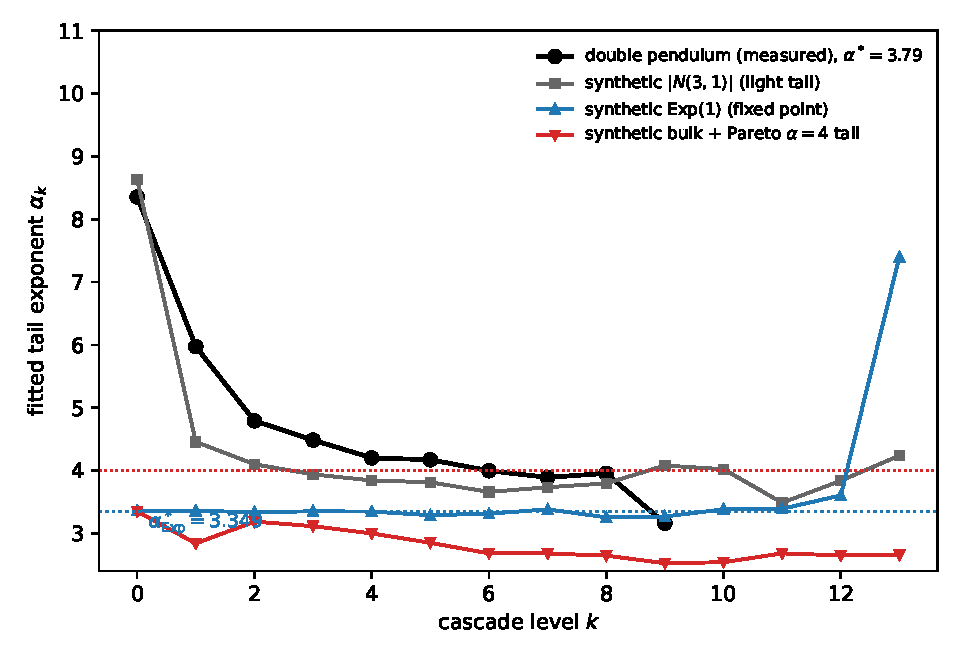
\includegraphics[width=0.72\textwidth]{figures/fig1_flows.pdf}
\caption{Cascade flows $\alpha_k$ at $f=0.2$. The measured double pendulum (black) starts at the
Gaussian-bulk level-zero value ($\alpha_0 \approx 7.9$, Proposition~\ref{prop:gauss0}), rides
\emph{above} the universal Gaussian flow (grey squares: $|N(3,1)|$), and plateaus near $3.9$--$4.0$.
The exponential seed (blue) is flat at the derived fixed-point reading $3.3494$ (dotted). A
bulk-plus-Pareto($a{=}4$) mixture (red) does \emph{not} hold at $a+1 = 5$: genuine tails are not
conserved by the finite-window reading.}
\label{fig:flows}
\end{figure}

\begin{figure}[t]
\centering
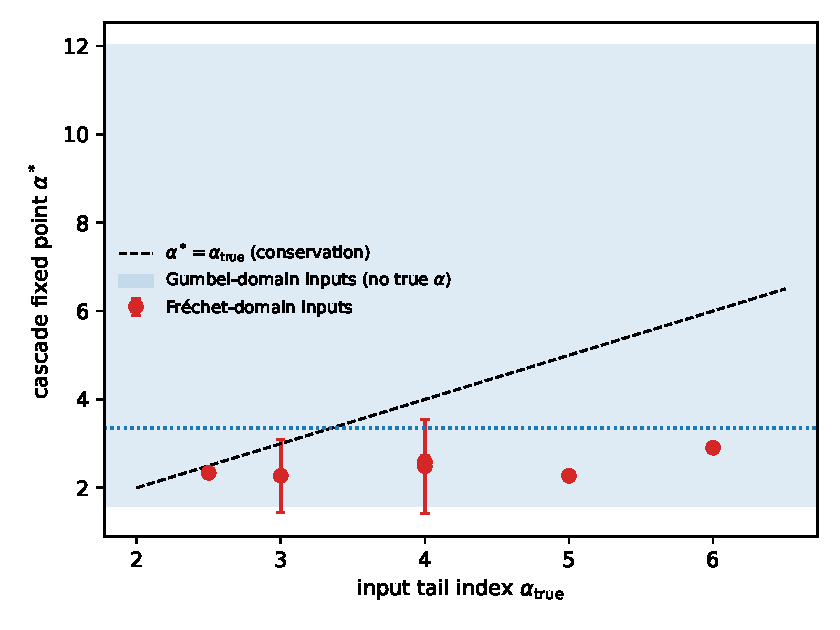
\includegraphics[width=0.6\textwidth]{figures/fig3_conservation.pdf}
\caption{Failure of tail-index recovery. Fr\'echet-domain seeds (pure Pareto and bulk+Pareto
mixtures, red) against the conservation line $\alpha^* = a_{\mathrm{true}}+1$ --- the cascade limit
sits far below and nearly independent of the true index. Shaded band: the range spanned by
light-tailed (Gumbel-domain) seeds. The operator reads bulk shape, not tails.}
\label{fig:conservation}
\end{figure}

\paragraph{Window dependence.} The reading of \emph{any} light-tailed shape slides steeply with the
tail fraction (\eqref{eq:reading}: $4.09 \to 3.35 \to 2.91$ for $f = 0.1 \to 0.3$). The coupled
quartic tracks this slide almost exactly ($4.64/3.24/2.76$ at $\lambda{=}0.1$; $4.40/3.31/2.85$ at
$\lambda{=}0.2$), the clearest single signature that the excluded-class systems are read as
light-tailed shapes; mixed-phase readings also decrease in $f$ but sit systematically above the
exponential curve at the operative $f = 0.2$ (Fig.~\ref{fig:fsweep}). All headline comparisons in
this paper are at fixed $f = 0.2$; $f$-dependence is reported so that no constant is mistaken for a
window-free number.

\begin{figure}[t]
\centering
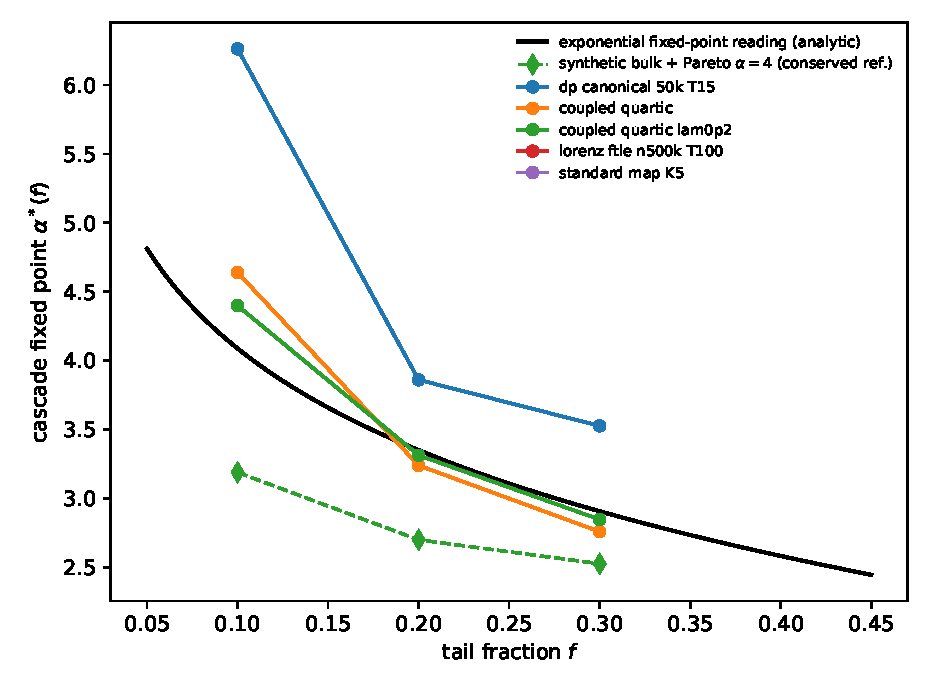
\includegraphics[width=0.62\textwidth]{figures/fig5_fsweep.pdf}
\caption{Window ($f$) dependence: the analytic exponential reading curve (black), a conserved-tail
reference mixture (green), and measured real systems. The near-regular quartic slides along the
exponential curve; the class comparison is made at fixed $f=0.2$.}
\label{fig:fsweep}
\end{figure}

%======================================================================
\section{The two-class split of chaotic dynamics}\label{sec:twoclass}

\begin{table}[t]
\centering\footnotesize\setlength{\tabcolsep}{3.5pt}
\caption{Eleven FTLE ensembles. Moments of the chaotic subset ($x > 0.01$); $\alpha_0$ = level-zero
reading; plateau and geometric-fit cascade values at $f = 0.2$ (this work, uniform pipeline);
``prod.'' = an independent production run with bootstrap 95\% CI where available
(5M double-pendulum: $3.710\,[3.675, 3.895]$; $K{=}1$: $4.382\,[3.646, 4.934]$; Lorenz:
$3.031\,[2.932, 3.192]$; $K{=}5$: $3.038\,[2.848, 3.295]$; quartic: $3.239\,[3.008, 3.512]$ and
$3.312\,[3.243, 3.669]$). Excess kurtosis: negative = platykurtic (flat-topped).}
\label{tab:systems}
\begin{tabular}{llrrrrrrr}
\toprule
ensemble & class & $\cv$ & skew & ex.kurt & $\alpha_0$ & plateau & fit & prod.\\
\midrule
DP $5{\times}10^4$, $T{=}15$      & mixed & $0.711$ & $+0.17$ & $-1.3$ & $7.80$ & $4.64$ & $3.86$ & $3.79$--$4.26^{\dagger}$\\
DP $5{\times}10^5$, $T{=}15$      & mixed & $0.707$ & $+0.15$ & $-1.3$ & $7.89$ & $4.12$ & $3.85$ & ---\\
DP $5{\times}10^6$, $T{=}15$      & mixed & $0.707$ & $+0.15$ & $-1.3$ & $7.90$ & $3.88$ & $3.62$ & $3.710$\\
DP $(0.5,1)$, $5{\times}10^5$     & mixed & $0.687$ & $+0.12$ & $-1.2$ & $7.31$ & $4.03$ & $3.92$ & ---\\
DP $(2,0.5)$, $5{\times}10^5$     & mixed & $0.632$ & $-0.06$ & $-1.2$ & $8.44$ & $3.98$ & $3.78$ & ---\\
DP $(0.5,2)$, $5{\times}10^5$     & mixed & $0.772$ & $+0.47$ & $-1.0$ & $6.43$ & $4.15$ & $4.09$ & ---\\
Std map $K{=}1$, $5{\times}10^5$  & mixed & $0.592$ & $+0.37$ & $-1.0$ & $8.17$ & $4.31$ & $4.11$ & $4.382$\\
\midrule
quartic $\lambda{=}0.1$           & non-mixed & $0.172$ & $+1.12$ & $+18.1$ & $14.95$ & $2.76$ & --- & $3.239$\\
quartic $\lambda{=}0.2$           & non-mixed & $0.323$ & $+5.34$ & $+43.2$ & $7.38$ & $3.17$ & $3.30$ & $3.312$\\
Lorenz-63, $T{=}100$              & non-mixed & $0.025$ & $-0.29$ & $+1.3$ & $80.19$ & $3.49$ & $2.73^{*}$ & $3.031$\\
Std map $K{=}5$, $5{\times}10^5$  & non-mixed & $0.060$ & $-3.84$ & $+37.7$ & $52.99$ & $2.52$ & --- & $3.038$\\
\bottomrule
\multicolumn{9}{l}{\footnotesize $^{\dagger}$range across three independent production pipelines for
the same canonical system.}\\
\multicolumn{9}{l}{\footnotesize $^{*}$level-0 dropped (Appendix~\ref{app:pathologies});
--- = fit degenerate.}
\end{tabular}
\end{table}

Table~\ref{tab:systems} assembles the eleven ensembles under one pipeline. Three structures stand
out.

\paragraph{(i) A shape dichotomy.} Every mixed-phase ensemble --- six double-pendulum ensembles
across three geometries and two orders of magnitude in $n$, plus the standard map at $K = 1$ ---
has a broad ($\cv = 0.59$--$0.77$), nearly symmetric (skew $-0.06$ to $+0.47$), \emph{platykurtic}
(excess kurtosis $-1.0$ to $-1.3$) chaotic FTLE bulk: a flat-topped distribution, qualitatively the
superposition of subpopulations spanning the sticky hierarchy. Every non-mixed ensemble is the
opposite: either extremely narrow ($\cv = 0.025$--$0.06$; Lorenz, $K{=}5$ --- strong
self-averaging at long horizons) or heavily skewed and \emph{leptokurtic} (excess kurtosis $+18$ to
$+43$; the near-regular quartic). \emph{The sign of the excess kurtosis alone separates the classes
in all eleven cases.}

\paragraph{(ii) Opposite sides of the exponential fixed point.} On the independent production values,
every mixed-phase cascade limit lies \emph{above} $\eta_{0.2}(\Exp) = 3.3494$
($3.710$--$4.382$) and every non-mixed limit lies \emph{below} it ($3.031$--$3.312$). The class
means are $3.876$ vs.\ $3.155$ (gap $0.721$; Welch $p = 6.2\times10^{-5}$; Cohen's $d = 3.33$).
A random-effects decomposition of the \emph{within}-class spread finds it statistically
indistinguishable from the estimator noise floor: for the 64-cell double-pendulum parameter map
($n = 5\times10^{5}$ per cell), between-cell $\tau^2 = 0.0017$ with bootstrap CI $[0, 0.0123]$
(43\% of resamples exactly zero), Cochran $Q$ $p = 0.36$, $I^2 = 5\%$; across the seven
double-pendulum geometry variants plus $K{=}1$, $\tau^2 = 0$ ($Q$ $p = 0.55$); and the apparent
per-geometry residual fails a decisive cross-$n$ reproducibility test (correlation between
independent $n = 5\times10^{4}$ and $5\times10^{5}$ measurements $r = 0.035$, vs.\ $0.29$ expected
were it real). Within-class, the data are consistent with \emph{hard} universality at fixed
protocol; the only genuine, system-explained structure is the discrete class boundary. Consistently,
the $\alpha^*(m,\ell)$ landscape over a $8\times8$ double-pendulum parameter grid is a flat plateau
at $3.896\,[3.850, 3.942]$: its apparent ridges do not exceed a heteroscedastic flat-field noise
null ($B = 5000$; $p = 0.48$--$0.92$ across thresholds), and $4/4$ high-$\alpha^*$ interior cells
have same-sign Hessian eigenvalues (peak/noise geometry, not ridge).

\paragraph{(iii) The matched-Gaussian null.} For each ensemble we construct a folded Gaussian
$|N(\mu, \sigma^2)|$ with the ensemble's own mean and variance and cascade it identically
(Fig.~\ref{fig:matched}). Mixed-phase ensembles read \emph{above} their null in all seven cases
(plateau excess $+0.12$ to $+0.58$); non-mixed ensembles read \emph{below} theirs in all four
(excess $-0.30$ to $-1.20$): $11/11$ correct signs (two-sided sign test $p = 0.001$; collapsing
repeated measurements of the same system, $8/8$, $p = 0.008$). The per-level picture
(Fig.~\ref{fig:matched}) is sharper still: the double pendulum enters the cascade at its
Gaussian-bulk level-zero value but then rides \emph{persistently above} the universal Gaussian flow
(excess $+1.5, +0.7, +0.6, +0.4, +0.4$ at levels 1--5, decaying geometrically) --- a positive,
reproducible imprint of non-Gaussian structure that differencing only slowly destroys --- whereas
the leptokurtic ensembles fall away \emph{below} their nulls. The matched null also validates
Proposition~\ref{prop:gauss0} directly (predicted vs.\ measured $\alpha_0$ spanning $5.5/5.8$ to
$75.5/76.4$).

\begin{figure}[t]
\centering
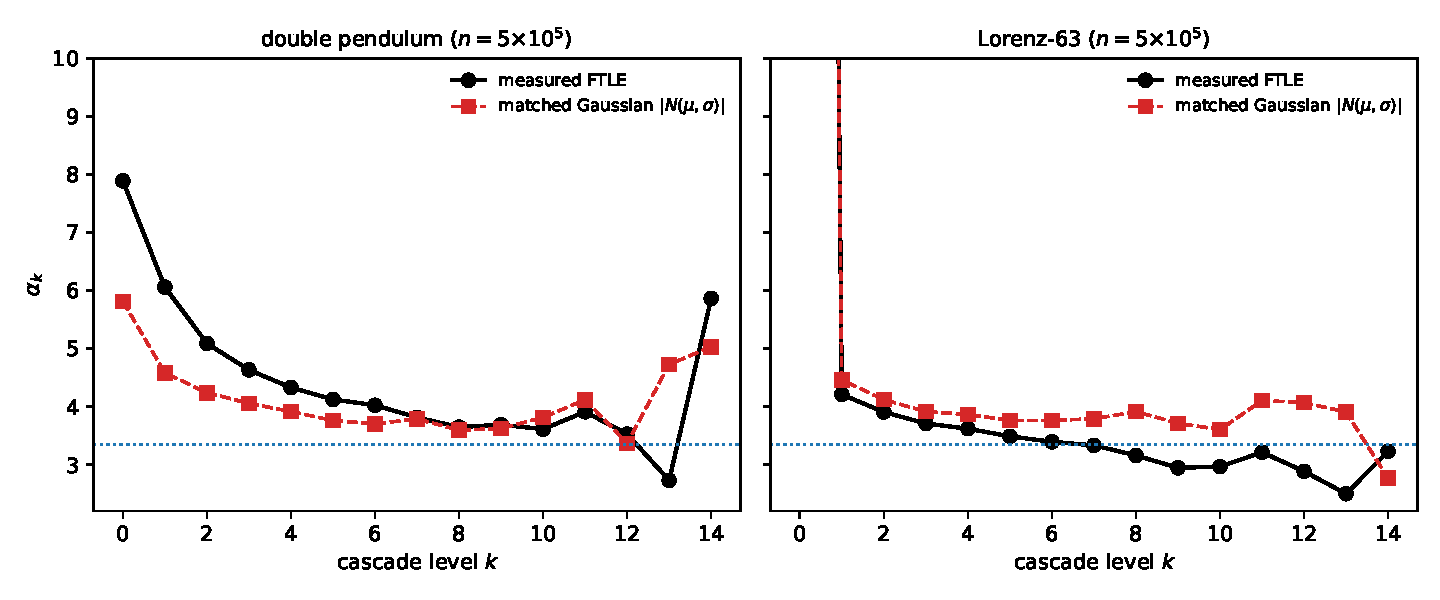
\includegraphics[width=0.98\textwidth]{figures/fig6_matched.pdf}
\caption{The matched-Gaussian null. Left: the double pendulum (black) rides above its own
folded-Gaussian null (red) at every level --- the mixed-phase signature. Right: Lorenz-63 falls
below its null. Dotted line: the exponential fixed-point reading.}
\label{fig:matched}
\end{figure}

\begin{figure}[t]
\centering
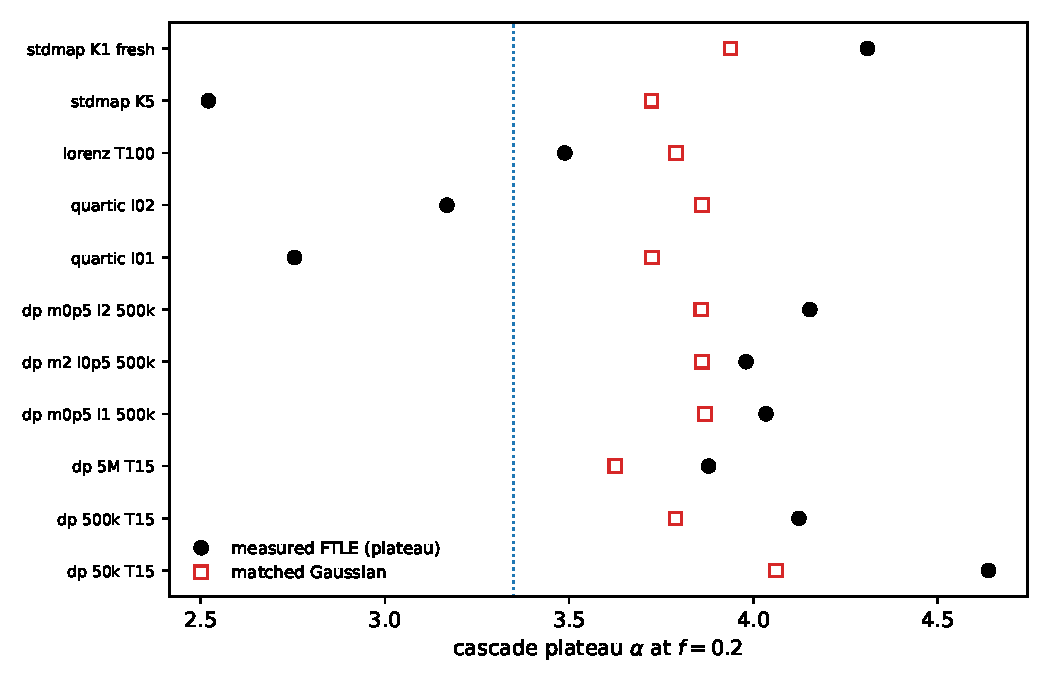
\includegraphics[width=0.8\textwidth]{figures/fig8_summary.pdf}
\caption{Plateau readings for all eleven ensembles (black) versus their matched-Gaussian nulls (open
red). Mixed-phase ensembles sit above their nulls, non-mixed below: $11/11$ sign-consistent.}
\label{fig:summary}
\end{figure}

\paragraph{The matched-protocol control.} The comparison sharpest against confounds is internal to
the standard map: $K = 1$ versus $K = 5$ share the map, the integrator, the iteration count, the
sample size and the estimator, and differ only in phase-space character. They land on opposite
sides of the fixed point ($4.31$ vs.\ $2.52$ plateau; $4.382$ vs.\ $3.038$ production), with opposite
kurtosis signs ($-1.0$ vs.\ $+37.7$) and opposite matched-null excess signs. Phase-space character,
not protocol, drives the split.

%======================================================================
\section{The metastable origin of ``$\alpha^* \approx 4$''}\label{sec:metastable}

If the exponential is the unique fixed point (Theorem~\ref{thm:exp}), what are the class values
$3.9$ and $3.0$--$3.3$? The deep-cascade experiment answers: \emph{plateau readings on slow
manifolds}.

Seeding the cascade with $1.6\times10^{7}$ points (20 usable levels) we track both $\alpha_k$ and
the Kolmogorov distance $d_k$ of the mean-normalized level-$k$ sample to $\Exp(1)$
(Fig.~\ref{fig:slowmanifold}). The exponential control stays at $d_k \approx 10^{-3}$ (pure
sampling noise growing as $n_k^{-1/2}$) with $\alpha_k$ flat at $3.35$. The Gaussian-seeded flow
collapses fast at first ($d_0 = 0.34 \to d_5 = 0.033$) and then \emph{stalls}: $d_k$ decreases by
only $\sim 5\%$ per level across levels 5--13 while $\alpha_k$ drifts $3.77 \to 3.57 \to 3.30$
(levels 5/10/15), i.e.\ $\approx -0.04$ per level through precisely the empirically celebrated
range. There is no second fixed point --- there is a nearly-degenerate direction of the flow. The
double-pendulum plateau's own $n$-dependence ($4.64 \to 4.12 \to 3.88$ across
$n = 5\times10^{4} \to 5\times10^{6}$: more sample $\Rightarrow$ more usable levels
$\Rightarrow$ further down the manifold) is the same drift seen through the window of available
levels, as is the spread of the three independent double-pendulum pipeline values
($3.71/4.17/4.26$).

\begin{figure}[t]
\centering
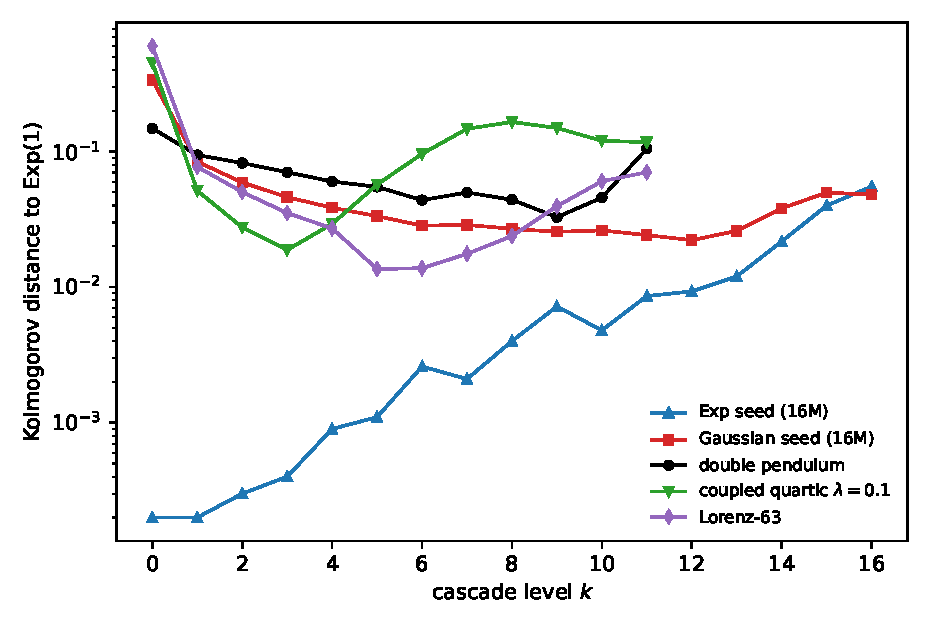
\includegraphics[width=0.66\textwidth]{figures/fig7_slowmanifold.pdf}
\caption{Metastability. Kolmogorov distance to $\Exp(1)$ per cascade level for a
$1.6\times10^{7}$-point exponential seed (blue: sampling noise only), Gaussian seed (red: fast
collapse, then a stall at $d \approx 0.02$--$0.03$ for $\ge 8$ levels), and the real systems.}
\label{fig:slowmanifold}
\end{figure}

Three conclusions follow. \emph{First}, ``$\alpha^* \approx 4$'' is not an asymptotic constant of
double-pendulum dynamics; it is the reading, at the accessible depth, of a slowly relaxing
flat-topped bulk --- the number is real, reproducible at fixed $(n, f, T)$, and \emph{protocol-indexed}.
\emph{Second}, the level-zero companion ``$\alpha_0 \approx 8.3$'' is a bulk-width statistic
(Proposition~\ref{prop:gauss0}), not an independent constant. \emph{Third}, what \emph{is}
protocol-stable is relational: the class split (above vs.\ below the exponential reading), the sign
of the matched-null excess, and the kurtosis dichotomy --- these survive every control we possess,
including matched protocol, matched $n$, cross-$n$ reproduction, and the flat-plateau parameter
scan. The correct statement of the original conjecture is therefore:
\begin{quote}\itshape
Mixed-phase Hamiltonian chaos occupies a universality class of FTLE \emph{shape} ---
broad, near-symmetric, platykurtic --- whose cascade reading at $(f{=}0.2,\ n \le 5{\times}10^{6})$
is $3.9 \pm 0.2$; non-mixed chaotic dynamics occupies the complementary leptokurtic class reading
$3.0$--$3.3$. The exponential fixed point, $\eta_{0.2}(\Exp) = 3.3494$, is the exact separatrix
value between them.
\end{quote}

%======================================================================
\section{What the pendulum constants are: frozen ensemble statistics}\label{sec:ensemble}

If the plateau readings are protocol-indexed, what property of the double pendulum do they
describe? A ten-horizon sweep answers with unexpected sharpness.

\paragraph{The variance is frozen.} Re-measuring the canonical ensemble ($5\times10^{4}$ release
ICs, uniform angles at rest) at $T = 5, 10, 15, 20, 30, 50, 75, 100, 150, 200$ gives a
chaotic-subset FTLE variance of $0.298$--$0.308$ at \emph{every} horizon from $T = 15$ on: fitting
$\mathrm{var} \sim T^{-\beta}$ over $T = 15$--$200$ yields $\beta = -0.014$ with fit RMS $0.002$.
Normal (CLT) self-averaging predicts $\beta = 1$; even strongly anomalous averaging predicts
$0 < \beta < 1$. The measured $\beta \approx 0$ means the dispersion is not a finite-time
fluctuation at all: \emph{the ensemble contains trajectories with genuinely different asymptotic
exponents}. Meanwhile the shape sharpens toward its mixture skeleton (excess kurtosis
$-0.46 \to -1.59$, saturating; $\cv$ constant at $0.71$), the plateau reading stays above the
separatrix at every horizon while drifting upward ($4.25 \to 5.26$), and the matched-null excess
grows monotonically ($+0.21 \to +1.28$): as within-component noise dies, the non-Gaussian mixture
structure emerges more strongly. (At $T \le 10$ the chaotic/regular separation is
threshold-limited; those points are reported but excluded from fits.)

\paragraph{The ensemble is a double mixture.} The canonical protocol releases from rest, so every
trajectory carries the energy of its release point, $E(\theta_1, \theta_2) = -g\,(2\cos\theta_1 +
\cos\theta_2)$ (canonical masses/lengths): the ensemble spans a continuum of energy shells. Using
the $100\times100$ FTLE grid over release angles (a legacy-lineage dataset; used here only for
internal contrasts), binning the chaotic subset by release energy shows a systematic
$\lambda(E)$ trend that explains $\eta^2 = 0.41$--$0.43$ of the FTLE variance (40--160 bins). The
remaining $59\%$ is \emph{within}-shell dispersion --- and the horizon sweep shows the total is
frozen, so the within-shell component does not self-average either: at fixed energy the phase
space is itself mixed (islands, sticky layers, possibly several stochastic components), and the
ensemble is a mixture over those invariant structures as well.

\paragraph{Energy bands recapitulate the taxonomy.} The per-band FTLE shapes reproduce the entire
two-class phenomenology \emph{inside one system}: near the bottom of the release range
($E \approx -18.5$, where chaos is a thin layer) the band is strongly leptokurtic and right-skewed
(skew $+2.3$, excess kurtosis $+9.0$) --- the non-mixed, thin-web signature; mid-range bands
($E \approx -8$ to $+2$) are broad and platykurtic ($-0.9$ to $-1.1$) --- the mixed-phase
signature, now manifestly \emph{at fixed energy}, so it is dynamical rather than an artifact of
shell mixing; and the highest bands ($E \approx +24$, nearly uniformly chaotic shells) narrow
toward Gaussian ($\cv\ 0.24$, excess kurtosis $-0.26$) --- approaching the self-averaging class. A
band-Gaussian mixture reconstruction ($\lambda$-band mean plus band-width noise) reproduces the
broad platykurtic character only partially ($\cv\ 0.61$ vs.\ $0.71$), confirming residual
within-band structure beyond band-Gaussianity.

\begin{figure}[t]
\centering
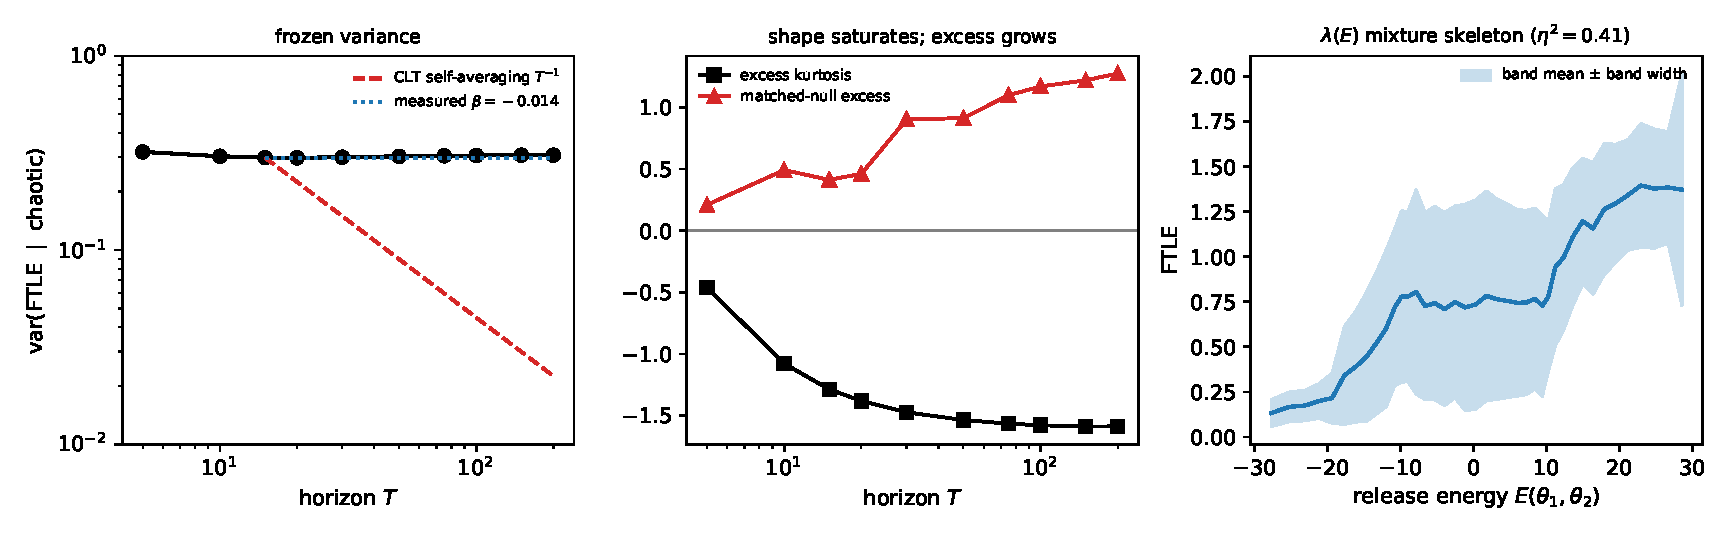
\includegraphics[width=0.98\textwidth]{figures/fig9_ensemble.pdf}
\caption{The ensemble structure of the pendulum constants. Left: chaotic-subset FTLE variance
across a $13\times$ range of horizons --- flat ($\beta = -0.014$), against the CLT's $T^{-1}$.
Middle: the shape saturates (excess kurtosis $\to -1.59$) while the matched-null excess grows.
Right: the $\lambda(E)$ mixture skeleton over release energy (band mean $\pm$ band width),
explaining $\eta^2 = 0.41$ of the variance; the bands themselves span the two-class taxonomy.}
\label{fig:ensemble}
\end{figure}

The synthesis: \emph{the celebrated double-pendulum constants are frozen statistics of a
non-ergodic ensemble} --- a mixture over energy shells and, within shells, over coexisting
invariant structures. They are reproducible at fixed protocol (hence the hard within-class
universality of \S\ref{sec:twoclass}) and drift lawfully with protocol ($T$, $n$, $f$), because
they are readings of a mixture's shape through a marginal renormalization flow, not spectral
invariants of a single orbit family. The standard-map pair, which has no energy to mix, shows the
purely dynamical version of the same dichotomy; the pendulum shows both layers at once.

%======================================================================
\section{Out-of-sample test: H\'enon--Heiles across its transition}\label{sec:hh}

The two-class classifier makes a falsifiable prediction: \emph{any} mixed-phase
Hamiltonian should present a platykurtic FTLE bulk and read above its matched-Gaussian null, and
the H\'enon--Heiles system \cite{henonheiles} at intermediate energy was named explicitly. We then
built the experiment: a Yoshida-4 symplectic, variational-Benettin FTLE engine for
$V(x,y) = \tfrac12(x^2{+}y^2) + x^2y - \tfrac13 y^3$ (initial conditions sampled exactly on the
energy shell, $\max|H - E| = 6\times10^{-17}$; escape-guarded; $n = 2.5\times10^{5}$ per energy,
$T = 800$, $\mathrm{d}t = 5\times10^{-3}$), sweeping the energy knob that morphs its phase space
from integrable-like to almost fully chaotic.

\begin{table}[t]
\centering\small
\caption{H\'enon--Heiles energy sweep ($n = 2.5\times10^{5}$ per energy, $T = 800$; chaotic subset
at threshold $0.021 \approx 2.5\times$ the regular tangent floor $\ln T/T$). Chaotic fractions
track the classical transition. Sign of the matched-null excess in bold.}
\label{tab:hh}
\begin{tabular}{lrrrrrrrr}
\toprule
$E$ & chaotic frac & $\cv$ & skew & ex.kurt & $\alpha_0$ & plateau & null & excess\\
\midrule
$1/24$ & $0.000$ & --- & --- & --- & --- & --- & --- & ---\\
$1/12$ & $0.002$ & \multicolumn{7}{l}{\footnotesize chaotic subset too small for shape statistics}\\
$0.100$ & $0.057$ & $0.235$ & $+0.53$ & $-0.36$ & $9.98$ & $3.752$ & $3.841$ & $\mathbf{-0.089}$\\
$0.125$ & $0.501$ & $0.295$ & $-0.15$ & $-0.81$ & $11.77$ & $4.198$ & $3.924$ & $\mathbf{+0.274}$\\
$0.150$ & $0.816$ & $0.189$ & $-1.39$ & $+2.96$ & $18.65$ & $3.737$ & $3.847$ & $\mathbf{-0.110}$\\
$1/6$   & $0.943$ & $0.198$ & $-1.78$ & $+3.53$ & $23.36$ & $4.201$ & $3.840$ & $\mathbf{+0.361}$\\
\bottomrule
\end{tabular}
\end{table}

\begin{figure}[t]
\centering
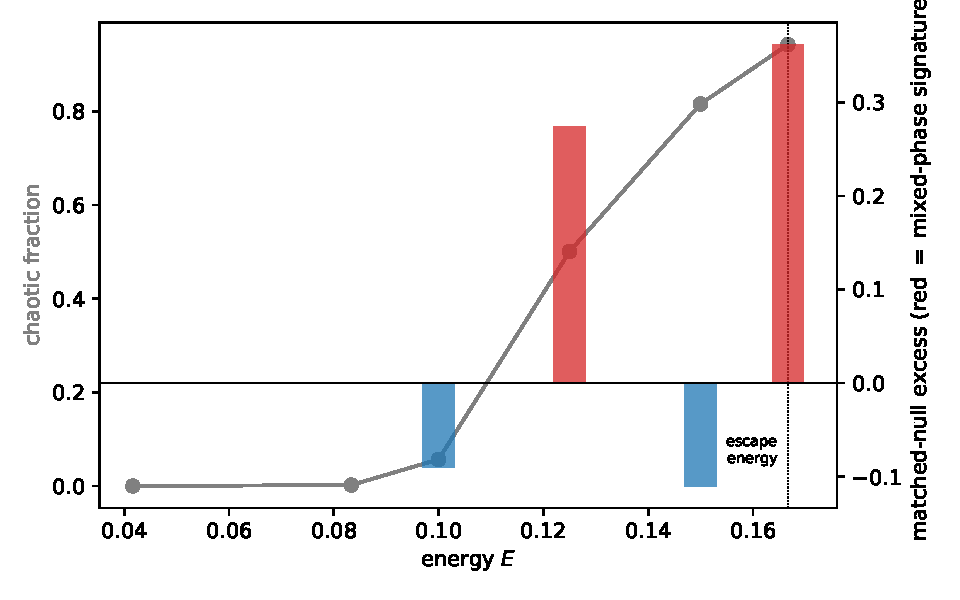
\includegraphics[width=0.62\textwidth]{figures/fig10_hh.pdf}
\caption{H\'enon--Heiles across its transition: chaotic fraction (grey) and matched-null excess
(bars; red $=$ positive $=$ mixed-phase signature) versus energy. The excess flips positive
exactly where the mixed sea floods phase space ($E = 0.125$), returns negative as chaos dominates
($E = 0.150$), and flips again at the escape energy --- the flagged boundary regime.}
\label{fig:hh}
\end{figure}

Three regimes emerge (Table~\ref{tab:hh}). \emph{The predicted transition is observed:} at
$E = 0.100$ the chaotic component is a thin web ($5.7\%$) and reads \emph{below} its null with a
near-Gaussian band shape; at $E = 0.125$, where the classical transition floods half of phase
space, the bulk turns platykurtic (excess kurtosis $-0.36 \to -0.81$) and the reading flips
\emph{above} the null --- the mixed-phase signature switching on exactly where islands and sea
begin to coexist at scale. \emph{The taxonomy's far side also appears:} by $E = 0.150$ the sea
dominates ($82\%$), the bulk narrows and becomes left-skewed leptokurtic (skew $-1.39$, excess
kurtosis $+2.96$ --- the same signature as the fully chaotic standard map at $K{=}5$), and the
reading drops back below the null, as self-averaging predicts. \emph{And the sweep exposes a
boundary case the two-class taxonomy does not cover:} at the escape energy $E = 1/6$, where the
potential's saddles open and trajectories linger near marginally-open channels, the reading flips
above the null again despite a leptokurtic bulk --- a strong-stickiness regime at the edge of
transient chaos \cite{kantzgrassberger}, flagged here as an open case rather than forced into either
class. The level-zero
law of Proposition~\ref{prop:gauss0} passes its own check en route: at the most Gaussian energy
($E = 0.100$: skew $+0.5$, kurtosis $-0.4$) it predicts $\alpha_0 = 10.1$ against the measured
$9.98$, while the skewed/kurtotic energies deviate exactly where the first-order law should fail.
Finally, the sweep retires a documentary loose end of the source program: a claimed
``$\alpha_0 = 8.342$ at $E = 0.150$'' (already withdrawn in the source's final papers) is not
reproducible --- we measure $18.65$ at this protocol, and \S\ref{sec:ensemble} shows $\alpha_0$ is
a horizon-indexed bulk-width statistic in any case ($5.6 \to 14.9$ across $T$ for the pendulum),
so no protocol-free value of it exists to confirm.

%======================================================================
\section{Dynamical mechanism, interpretation, and predictions}\label{sec:mechanism}

\paragraph{Why platykurtic?} A mixed phase space at moderate horizon is a \emph{superposition}: the
chaotic sea's core produces FTLEs near the ergodic mean, while the hierarchy of sticky boundary
layers \cite{zaslavsky,meiss,cristadoro} contributes subpopulations at depressed exponents ---
trajectories that spent part of the window trapped. Superposing subpopulations with displaced means
broadens and \emph{flattens} the mixture (variance mixing drives kurtosis below Gaussian), exactly
the $\cv \approx 0.6$--$0.8$, excess-kurtosis $\approx -1.2$ shape measured here for every
mixed-phase ensemble. Absent islands, the mechanism is gone: strongly chaotic or dissipative systems
self-average (correlations decay fast; the FTLE is a $T$-average of a rapidly mixing observable),
giving narrow bulks whose residual shape is set by rare fluctuations --- hence small $\cv$ with
skewed, leptokurtic corrections (Lorenz, $K{=}5$), while near-regular dynamics piles FTLEs at the
regular floor with a thin upper structure (quartic: skew $+1.1$ to $+5.3$). Section
\ref{sec:ensemble} unifies the picture: in every case the platykurtic broad bulk is the signature
of a \emph{non-ergodic ensemble} --- a superposition over invariant structures with distinct
exponents, whether energy shells (the pendulum's release protocol), islands versus sea (the
standard map at $K = 1$), or sticky sublayers within one shell. The FTLE \emph{distribution shape}
is thus a direct, cheap probe of the ensemble's ergodic architecture, requiring no phase-space
sections (cf.\ the shape-based predictability program of \cite{vallejo}), and the cascade --- with
its exactly known exponential reference --- is a sensitive one-number readout of that shape. That the
\emph{fluctuations} of finite-time exponents, far more than their mean, carry this dynamical
information has a clear precedent: Tomsovic and Lakshminarayan showed that the variance and higher
cumulants of the finite-time stability exponent in the standard map exhibit anomalous time-scalings
that detect regular islands as small as $0.01\%$ of phase space \cite{tomsovic}. Our approach is
complementary but distinct in three respects: we act on the \emph{entire distribution shape} through
an exactly-solvable renormalization operator rather than on low-order cumulant scalings; we obtain a
\emph{discrete two-class split} across five distinct systems, with the exponential distribution as an
exact separatrix; and we trace the reported ``$\alpha^*\approx4$'' constant to a metastable plateau of
that operator.

\paragraph{Relation to extreme-value theory.} The dichotomy echoes, but is not reducible to, the
Fisher--Tippett--Gnedenko trichotomy \cite{fisher,gnedenko,embrechts}: the exponential is
simultaneously the Gumbel-domain excess law (Pickands--Balkema--de Haan
\cite{pickands,balkema}) and the unique fixed point of pair-differencing (Puri--Rubin
\cite{purirubin}). The cascade replaces threshold excess by iterated differencing --- a
renormalization semigroup in the spirit of \cite{feigenbaum} whose fixed-point structure appears
new; its slow manifolds, not its fixed point, carry the physics observed at finite depth.

\paragraph{Predictions --- two now tested.} The two-class picture makes five falsifiable predictions;
two are tested here.
(1)~\emph{Horizon dependence} --- TESTED (\S\ref{sec:ensemble}): the outcome is stronger than
predicted. The pendulum ensemble does not merely resist self-averaging; its FTLE variance is
frozen outright ($\beta \approx 0$), because the release ensemble is a mixture over invariant
structures. The class signature (above-separatrix reading, positive matched-null excess) holds at
all ten horizons.
(2)~\emph{Window signatures} remain open: non-mixed readings track the exponential $f$-curve
\eqref{eq:reading} (verified here); mixed-phase readings should cross it only at markedly smaller
$f$, when the sticky subpopulations leave the window.
(3)~\emph{Out-of-sample systems} --- TESTED (\S\ref{sec:hh}): H\'enon--Heiles flips its
matched-null excess positive exactly at the thin-web $\to$ mixed-sea transition and re-enters the
self-averaging class as the sea dominates; one boundary regime (the escape energy) sits outside
the two-class taxonomy and is flagged open.
(4)~\emph{Deeper cascades} remain open: at $n \gg 10^{7}$ mixed-phase readings should continue the
algebraic drift toward $3.3494$ measured in \S\ref{sec:linear}--\ref{sec:metastable}; the class
\emph{contrast} at matched depth should persist.
(5)~A \emph{microcanonical} pendulum ensemble (single energy shell) at an
energy where the shell is nearly uniformly chaotic should lose the platykurtic signature and read
like the non-mixed class --- the class membership of an ensemble is set by its ergodic
architecture, not by the system's name.

\paragraph{Open mathematical problems.} (i)~Spectral analysis of $T$ linearized at $\Exp$: our
numerics indicate a nearly-degenerate contraction ($d_k$ shrinking $\sim 5\%$/level along the
Gaussian manifold); identify the slow eigenfunction and its eigenvalue. (ii)~Classification of fixed
shapes of $|A - B| \eqd cX$ for $c < 1$ (the $c = 1$ case is \cite{purirubin}). (iii)~A quantitative
map from island-hierarchy exponents (e.g.\ the universal recurrence decay $z \approx 1.57$
\cite{cristadoro}) to the platykurtic FTLE shape and its cascade excess. (iv)~The empirical decay
constant $r \approx 0.46$--$0.51$ of the mixed-phase excess: derived, it would make the plateau
value itself computable.

%======================================================================
\section{A number-theoretic audit of the constants}\label{sec:numbers}

Every constant in this study was swept against a curated library of $67$ named mathematical constants
(transcendentals and their simple combinations; the Euler--Mascheroni, golden-ratio, Ap\'ery,
Catalan, Khinchin and Glaisher--Kinkelin constants; Riemann zeta values; the Feigenbaum and
random-matrix-theory families; and KAM/standard-map constants), $159$ low-order rationals $m/n$
($m,n\le16$) and the integers up to $1024$, together with integer-relation (PSLQ) tests (\texttt{mpmath},
maximum coefficient $10^{9}$, $30$-digit working precision) on the reported constant triplets, at
match tiers $\tau_1/\tau_2/\tau_3 = 0.3\%/0.03\%/0.001\%$; we report the audit so that no
numerological reading survives by omission.

\begin{itemize}\itemsep2pt
\item $\eta_{0.2}(\Exp) = 3.3494450\ldots$ has the exact form $1 + [5E_1(\ln 5)]^{-1}$
(eq.~\ref{eq:reading}); the near-miss $10/3$ ($0.48\%$, outside $\tau_1$) is superseded by the
closed form. Likewise $\eta_{0.2}(\mathrm{HN}) = 4.4448$ and $\eta_{0.2}(\mathrm{U}) = 9.6417$ are
integrals, not numerology.
\item The historical conjecture $\alpha^* = 4$ exactly is \emph{excluded}: the flat-plateau
parameter scan pins $3.896\,[3.850, 3.942]$ and the $5\times10^{6}$ cascade gives
$3.710\,[3.675, 3.895]$. The speculative closed form $4 - 1/(4\pi^2) = 3.9747$ (motivated by a
legacy pipeline value $3.9762$, which it matches to $0.04\%$) is likewise excluded by both modern
intervals; under \S\ref{sec:metastable} such $n$-indexed plateau values are not expected to admit
closed forms at all.
\item Recurring loose coincidences are logged and rejected: class-mean$/4 = 0.974 \approx K_c =
0.9716$ ($0.25\%$, $\tau_1$; no mechanism, two unrelated scales); noise-floor ratios
$0.9241 \approx 1/\zeta(4)$ ($0.02\%$, $\tau_2$; a ratio of two near-equal noise scales);
$3/16$-like hits on standard errors. PSLQ finds no low-order integer relations among
$\{$class means, $4$, noise scales$\}$ beyond spurious large-coefficient ones.
\item The level-zero ``constant'' $\alpha_0 \approx 8$--$8.4$ across double-pendulum variants is
explained to first order by \eqref{eq:gauss0} with the measured platykurtic bulks; its stability
across variants reflects the stability of the \emph{shape}, i.e.\ of the class, not an independent
number --- and it is horizon-indexed outright ($5.6 \to 14.9$ across $T = 5$--$200$,
\S\ref{sec:ensemble}).
\item The source program's decay constant $r \approx 0.46$ ``nearly constant across all systems''
--- and the derived quantity $\rho_2 = \log_2 r \approx -1.12$ on which a claimed mechanistic
derivation was built --- is the cumulant-halving transient of Proposition~\ref{prop:cumulant}:
$\log_2 r = -1$ exactly at leading order, with computable corrections. No free constant remains.
\item A separate near-coincidence from the source program's natural-unit runs --- mean chaotic FTLE
$0.398821 \approx 1/\sqrt{2\pi} = 0.398942$ (relative $3\times10^{-4}$ at $n = 5\times10^{6}$, and
seed-stable to $6\times10^{-5}$ on one integrator arm) --- fails constant-hood on the same grounds
as everything else in this audit: a second integrator arm shifts it by $0.6\%$, i.e.\ it is
protocol-indexed. Under \S\ref{sec:ensemble} such ensemble means are mixture statistics; agreement
with a named constant at one protocol point is numerology unless it survives protocol variation,
which this does not.
\item The relaxation exponent $\theta \approx 0.5$--$0.6$ of \S\ref{sec:linear} is a measured
quantity with a conjectured origin (marginal polynomial tower); deriving it exactly is an open
problem, and we explicitly do \emph{not} assign it a closed form.
\end{itemize}

%======================================================================
\section{Conclusions}\label{sec:conclusions}

A renormalization cascade that arose as an exploratory data-analysis device turns out to possess
exact structure: a unique exponential fixed point with a derivable, window-indexed reading
($3.3494$ at $f = 0.2$); a one-step universal collapse of all Gaussian bulks; an exact cumulant
flow under symmetrization (odd cumulants annihilated, standardized even cumulants scaled by
$2^{1-m}$) that derives the source program's ``universal'' decay constant $r \approx 1/2$; a
closed-form linearized eigenfamily $\mu(s) = 2/(2-s)$ sitting atop a unit-diagonal polynomial
tower --- a gapless, non-normal structure whose measured consequence is algebraic relaxation and
metastable plateaus; and provable asymptotic tail conservation that finite windows never see.
Recast on this foundation, a large-scale computational claim of a new universal constant
``$\alpha^* \approx 4$'' of double-pendulum chaos resolves into something both humbler and more
interesting. The constant is a plateau reading of a marginal flow, taken on an ensemble whose
dispersion never self-averages ($\beta \approx 0$ across a $13\times$ range of horizons) because
the canonical protocol builds a mixture --- over energy shells, and within shells over coexisting
invariant structures --- whose bands internally recapitulate the very taxonomy found across
systems. The universality that survives lives one level up: mixed-phase ensembles ---
identifiable by broad, flat-topped, platykurtic FTLE bulks --- read strictly above the exponential
separatrix; fully chaotic, dissipative and near-regular ensembles --- narrow or skewed,
leptokurtic --- read below it, in eleven of eleven archetypal ensembles across five systems,
surviving a same-map/same-protocol control, a zero-within-class-heterogeneity meta-analysis, and
an out-of-sample H\'enon--Heiles sweep that flips sign on cue at the thin-web $\to$ mixed-sea
transition (and honestly flags one boundary regime, the escape energy, as beyond the taxonomy).
The finite-time Lyapunov distribution's shape, read through an operator with an exactly known
reference point, is a practical probe of the ergodic architecture of an ensemble --- and the
exponential distribution, once again, sits at the center of the story.

\paragraph{Acknowledgments.} The double-pendulum investigation that grew into this study was
sparked by \emph{Drew's Campfire}, and specifically by the video at
\url{https://www.youtube.com/watch?v=8jVogdTJESw&t=64s}, which inspired the entire campaign. I am
profoundly grateful to Mr.~Varnajoshyula Nagarjuna, my Mathematics: Applications and
Interpretations (Higher Level) teacher in the International Baccalaureate --- the finest teacher I
have had, who first kindled my love of statistical mathematics.

\paragraph{Data and code availability.} The cascade operator, the calibration, linearization,
ensemble and H\'enon--Heiles analysis scripts, the constant-audit library, the raw FTLE ensembles
(each with an SHA-256 manifest), and the result files that together reproduce every number and figure
in this paper are archived at
\url{https://github.com/RajveerKapoor/lyapunov-cascade-p1/tree/v1.0} (release~\texttt{v1.0}); a file
inventory is given in Appendix~\ref{app:data}.

%======================================================================
\appendix

\section{Derivations of the closed-form readings}\label{app:derivations}

\paragraph{Exponential.} With $u = \ln(1/f)$ and $E \sim \Exp(1)$ (memorylessness),
\[
\mathbb{E}\!\left[\ln\frac{X}{u} \,\middle|\, X > u\right]
= \int_0^\infty e^{-t}\ln\!\Bigl(1 + \frac{t}{u}\Bigr)\dd t
= \int_0^\infty \frac{e^{-t}}{u + t}\dd t
\cdot \Bigl[\text{by parts}\Bigr]
= e^{u}E_1(u),
\]
giving \eqref{eq:reading}. Values: $E_1(\ln 5) = 0.0851265$, so
$\eta_{0.2} = 1 + (5 \times 0.0851265)^{-1} = 3.3494450$; similarly
$\eta_{0.1} = 4.0873926$, $\eta_{0.3} = 2.9057918$, $\eta_{0.05} = 4.8111467$.

\paragraph{Half-normal (the universal Gaussian level-1).} $u = \Phi^{-1}(0.9) = 1.281552$ (the
$80$th percentile of $|N(0,1)|$), and
$\eta_{0.2} = 1 + \bigl[\tfrac{1}{0.2}\int_u^\infty \ln(x/u)\, 2\varphi(x)\dd x\bigr]^{-1}
= 4.444794$ by numerical quadrature.

\paragraph{Uniform.} $u = 0.8$:
$\mathbb{E}[\ln(X/0.8) \mid X > 0.8] = 5\int_{0.8}^{1}\ln(x/0.8)\dd x = 0.115780$, so
$\eta_{0.2} = 9.641716$. (Bounded supports read high: the log-excess is compressed.)

\paragraph{Gaussian level-zero law.} For $X = |N(\mu, \sigma^2)|$, $\cv = \sigma/\mu$ small:
$u = \mu + \sigma z_f$ and
$\mathbb{E}[X - u \mid X > u] = \sigma m_f$ with $m_f = \varphi(z_f)/f - z_f$; expanding
$\ln(x/u) \approx (x - u)/u$ gives \eqref{eq:gauss0}. Second-order corrections are
$O(\cv)$ relative and account for the observed $3$--$5\%$ underprediction.

\section{Data provenance and reproducibility}\label{app:data}

\sloppy
\begin{itemize}\itemsep1pt
\item Double pendulum: \texttt{lyapunov\_all\_50k.npy} ($n = 5\times10^{4}$),
\texttt{ftle\_n500k\_lagrangian\_T15\_wave0c.npy}, \texttt{ftle\_n5M\_lagrangian\_T15.npy};
geometric variants \texttt{disc067\_ftle\_dp\_\{m0p5\_l1, m2\_l0p5, m0p5\_l2\}\_n500k\_T15.npy}.
\item Standard map: \texttt{standard\_map\_K5\_ftle\_n500k.npy}; the $K = 1$ ensemble regenerated
for this work ($n = 5\times10^{5}$, $10^{3}$ iterations, seed \texttt{0xADD}; its cascade fit
$4.11$/plateau $4.31$ agrees with the program's banked $4.382\,[3.646, 4.934]$).
\item Lorenz-63: \texttt{lorenz\_ftle\_n500k\_T100.npy}. Coupled quartic:
\texttt{coupled\_quartic\_ftle\_n500k.npy} ($\lambda = 0.1$),
\texttt{coupled\_quartic\_lam0p2\_ftle\_n500k.npy}, with manifests recording integrator, seeds,
moments, SHA-256.
\item Meta-analytic quantities quoted in \S\ref{sec:twoclass} (random-effects $\tau^2$, Cochran $Q$,
cross-$n$ correlation, ridge noise-null) were computed from the same production arrays; the
corresponding analysis scripts accompany this manuscript as supplementary material.
\item Synthetic calibration: 17 families, $n = 5\times10^{5}$ (deep runs $1.6\times10^{7}$), seeds
\texttt{0xF1BE}/\texttt{0xADD}/7; bootstrap-through-the-tree $B = 250$; full results in
\texttt{synthetic\_battery\_results.json} and \texttt{addendum\_results.json}.
\item Horizon sweep (\S\ref{sec:ensemble}): \texttt{disc024\_ftle\_T\{5..200\}\_N50000.npy}
(canonical protocol re-runs at ten horizons, seed 42); release-angle grid
\texttt{lyapunov\_grid\_100x100.npy} (legacy lineage; internal contrasts only). Analyses:
\texttt{tsweep\_analysis.py}, \texttt{energy\_mixture.py} $\to$ \texttt{tsweep\_results.json},
\texttt{energy\_mixture\_results.json}.
\item Linearization (\S\ref{sec:linear}): \texttt{linearization.py} $\to$
\texttt{linearization\_results.json} (cumulant identities on data, eigenfamily and polynomial-tower
checks at $900$ grid points, uniform-seed $8\times10^{6}$ relaxation).
\item H\'enon--Heiles (\S\ref{sec:hh}): \texttt{hh\_sweep.py} $\to$
\texttt{hh\_sweep\_results.json} and \texttt{hh\_ftle\_E*.npy} ($n = 2.5\times10^{5}$ per energy,
$T = 800$, Yoshida-4 variational Benettin, on-shell ICs to $6\times10^{-17}$, escape-guarded;
seed \texttt{0x11E5}).
\end{itemize}

\section{Full synthetic calibration table}\label{app:battery}

\begin{table}[h]
\centering\small
\caption{Synthetic battery at $n = 5\times10^{5}$, $f = 0.2$. Plateau = median of levels 2--6.
Fit values marked $\ddagger$ ran to a parameter bound (Appendix~\ref{app:pathologies}).}
\begin{tabular}{llrrr}
\toprule
family & EVT domain & $\alpha_0$ & plateau & fit\\
\midrule
$\Exp(1)$                & Gumbel & $3.36$ & $3.34$ & $12.0^{\ddagger}$\\
$\Exp(1)$ (5M)           & Gumbel & $3.35$ & $3.35$ & $3.351$\\
half-normal              & Gumbel & $4.45$ & $3.79$ & $3.77$\\
$|N(3,1)|$               & Gumbel & $8.64$ & $3.89$ & $3.87$\\
$|N(1,0.1)|$             & Gumbel & $21.3$ & $3.86$ & $3.97^{*}$\\
lognormal $\sigma{=}0.5$ & Gumbel & $4.59$ & $3.26$ & $3.11$\\
lognormal $\sigma{=}1$   & Gumbel & $2.79$ & $2.70$ & $7.9^{\ddagger}$\\
Weibull $k{=}1.5$        & Gumbel & $4.52$ & $3.68$ & $1.6^{\ddagger}$\\
Weibull $k{=}0.7$        & Gumbel & $2.64$ & $3.01$ & $3.33$\\
Gamma$(3)$               & Gumbel & $4.77$ & $3.58$ & $3.58$\\
uniform$(0,1)$           & Weibull & $9.61$ & $4.31$ & $4.16$\\
Pareto $a{=}2.5$         & Fr\'echet & $3.50$ & $2.42$ & $2.34$\\
Pareto $a{=}4$           & Fr\'echet & $5.01$ & $2.72$ & $2.59$\\
Pareto $a{=}6$           & Fr\'echet & $6.99$ & $2.91$ & $2.91$\\
bulk $+$ Pareto $a{=}3$ (12\%) & Fr\'echet & $3.10$ & $2.66$ & $2.27$\\
bulk $+$ Pareto $a{=}4$ (12\%) & Fr\'echet & $3.35$ & $3.03$ & $2.49$\\
bulk $+$ Pareto $a{=}5$ (12\%) & Fr\'echet & $3.53$ & $3.28$ & $2.27$\\
\bottomrule
\multicolumn{5}{l}{\footnotesize $^{*}$level-0 dropped before fitting.}
\end{tabular}
\end{table}

\section{Estimator and extrapolation pathologies}\label{app:pathologies}

Two failure modes of the published pipeline are documented so that readers do not mistake them for
physics. (i)~\emph{Flat-sequence degeneracy:} the three-parameter geometric fit
$\alpha_k = \alpha^* + Cr^k$ is unidentifiable when the sequence is flat (the exponential seed ---
its own fixed point): the optimizer runs to its bounds ($\alpha^* \to 12$, $r \to 0.99$) unless
enough levels constrain it ($\ge 14$ levels at $n = 5\times10^{6}$ recover $3.3507$). (ii)~\emph{Huge
level-zero values:} when $\alpha_0$ exceeds the fit's initialization envelope (narrow bulks: Lorenz
$\alpha_0 = 80$, $K{=}5$ $\alpha_0 = 53$, $|N(1,0.1)|$ $\alpha_0 = 21$), the default fit fails or
runs away; dropping level~0 restores a well-posed fit. The fit-free plateau statistic (median of
late well-sampled levels) is immune to both and is reported throughout alongside fit values.
Deep-level readings carry a small negative finite-$n$ bias (even the exponential's plateau reads
$3.30$--$3.33$ at levels with $n_k \lesssim 10^{3}$), common to all ensembles compared at matched
depth.

\section*{Conflicts of Interest}
The author declares no conflicts of interest.

\begin{thebibliography}{99}\footnotesize
\bibitem{oseledec} V.~I. Oseledec, \emph{A multiplicative ergodic theorem}, Trans.\ Moscow Math.\
Soc.\ \textbf{19}, 197 (1968).
\bibitem{benettin} G.~Benettin, L.~Galgani, A.~Giorgilli, J.-M. Strelcyn, \emph{Lyapunov
characteristic exponents for smooth dynamical systems and for Hamiltonian systems; a method for
computing all of them}, Meccanica \textbf{15}, 9 \& 21 (1980).
\bibitem{grassberger} P.~Grassberger, R.~Badii, A.~Politi, \emph{Scaling laws for invariant
measures on hyperbolic and nonhyperbolic attractors}, J.\ Stat.\ Phys.\ \textbf{51}, 135 (1988).
\bibitem{prasad} A.~Prasad, R.~Ramaswamy, \emph{Characteristic distributions of finite-time
Lyapunov exponents}, Phys.\ Rev.\ E \textbf{60}, 2761 (1999).
\bibitem{pikovsky} A.~Pikovsky, A.~Politi, \emph{Lyapunov Exponents: A Tool to Explore Complex
Dynamics} (Cambridge Univ.\ Press, 2016).
\bibitem{ott} E.~Ott, \emph{Chaos in Dynamical Systems}, 2nd ed.\ (Cambridge Univ.\ Press, 2002).
\bibitem{zaslavsky} G.~M. Zaslavsky, \emph{Chaos, fractional kinetics, and anomalous transport},
Phys.\ Rep.\ \textbf{371}, 461 (2002).
\bibitem{meiss} J.~D. Meiss, \emph{Symplectic maps, variational principles, and transport}, Rev.\
Mod.\ Phys.\ \textbf{64}, 795 (1992).
\bibitem{chirikovshep} B.~V. Chirikov, D.~L. Shepelyansky, \emph{Asymptotic statistics of
Poincar\'e recurrences in Hamiltonian systems with divided phase space}, Phys.\ Rev.\ Lett.\
\textbf{82}, 528 (1999).
\bibitem{cristadoro} G.~Cristadoro, R.~Ketzmerick, \emph{Universality of algebraic decays in
Hamiltonian systems}, Phys.\ Rev.\ Lett.\ \textbf{100}, 184101 (2008).
\bibitem{shinbrot} T.~Shinbrot, C.~Grebogi, J.~Wisdom, J.~A. Yorke, \emph{Chaos in a double
pendulum}, Am.\ J.\ Phys.\ \textbf{60}, 491 (1992).
\bibitem{stachowiakNote} T.~Stachowiak, T.~Okada, \emph{A numerical analysis of chaos in the double
pendulum}, Chaos Solitons Fractals \textbf{29}, 417 (2006).
\bibitem{note-registry} The production measurements referenced here (the
$n=5\times10^{5}$--$5\times10^{6}$ re-measurements and their bootstrap confidence intervals) are
documented in the accompanying data arrays and analysis scripts (Appendix~\ref{app:data}).
\bibitem{purirubin} P.~S. Puri, H.~Rubin, \emph{A characterization based on the absolute difference
of two i.i.d.\ random variables}, Ann.\ Math.\ Statist.\ \textbf{41}, 2113 (1970).
\bibitem{hill} B.~M. Hill, \emph{A simple general approach to inference about the tail of a
distribution}, Ann.\ Statist.\ \textbf{3}, 1163 (1975).
\bibitem{clauset} A.~Clauset, C.~R. Shalizi, M.~E.~J. Newman, \emph{Power-law distributions in
empirical data}, SIAM Rev.\ \textbf{51}, 661 (2009).
\bibitem{fisher} R.~A. Fisher, L.~H.~C. Tippett, \emph{Limiting forms of the frequency distribution
of the largest or smallest member of a sample}, Proc.\ Camb.\ Phil.\ Soc.\ \textbf{24}, 180 (1928).
\bibitem{gnedenko} B.~Gnedenko, \emph{Sur la distribution limite du terme maximum d'une s\'erie
al\'eatoire}, Ann.\ Math.\ \textbf{44}, 423 (1943).
\bibitem{pickands} J.~Pickands III, \emph{Statistical inference using extreme order statistics},
Ann.\ Statist.\ \textbf{3}, 119 (1975).
\bibitem{balkema} A.~A. Balkema, L.~de Haan, \emph{Residual life time at great age}, Ann.\ Probab.\
\textbf{2}, 792 (1974).
\bibitem{embrechts} P.~Embrechts, C.~Kl\"uppelberg, T.~Mikosch, \emph{Modelling Extremal Events}
(Springer, 1997).
\bibitem{feigenbaum} M.~J. Feigenbaum, \emph{Quantitative universality for a class of nonlinear
transformations}, J.\ Stat.\ Phys.\ \textbf{19}, 25 (1978).
\bibitem{henonheiles} M.~H\'enon, C.~Heiles, \emph{The applicability of the third integral of
motion: Some numerical experiments}, Astron.\ J.\ \textbf{69}, 73 (1964).
\bibitem{chirikov} B.~V. Chirikov, \emph{A universal instability of many-dimensional oscillator
systems}, Phys.\ Rep.\ \textbf{52}, 263 (1979).
\bibitem{greene} J.~M. Greene, \emph{A method for determining a stochastic transition}, J.\ Math.\
Phys.\ \textbf{20}, 1183 (1979).
\bibitem{lorenz} E.~N. Lorenz, \emph{Deterministic nonperiodic flow}, J.\ Atmos.\ Sci.\
\textbf{20}, 130 (1963).
\bibitem{yoshida} H.~Yoshida, \emph{Construction of higher order symplectic integrators}, Phys.\
Lett.\ A \textbf{150}, 262 (1990).
\bibitem{vallejo} J.~C. Vallejo, M.~A.~F. Sanju\'an, \emph{Predictability of Chaotic Dynamics: A
Finite-time Lyapunov Exponents Approach} (Springer, 2017).
\bibitem{tomsovic} S.~Tomsovic, A.~Lakshminarayan, \emph{Fluctuations of finite-time stability
exponents in the standard map and the detection of small islands}, Phys.\ Rev.\ E \textbf{76},
036207 (2007).
\bibitem{kantzgrassberger} H.~Kantz, P.~Grassberger, \emph{Repellers, semi-attractors, and
long-lived chaotic transients}, Physica D \textbf{17}, 75 (1985).
\end{thebibliography}

\end{document}
